\section{Results}
\label{sec:results}
The results are organised as follows. The clustering and neural-network metrics refer to the finest grid, which is the one used for training, whereas the embedded ML-based RANS model is evaluated on the coarser grids, which are never used during training. This separation is intentional: it allows the embedded closure to be assessed strictly out of sample and shows that its benefit over the standard RANS model is twofold, in accuracy and in computational cost.

\subsection{Clustering results}
\label{sec:clustering_results}
First of all the PCA results are shown in Fig.~\ref{fig:pca}. 
\begin{figure}[h]
    \centering
    \begin{subfigure}{0.49\textwidth}
        \centering
        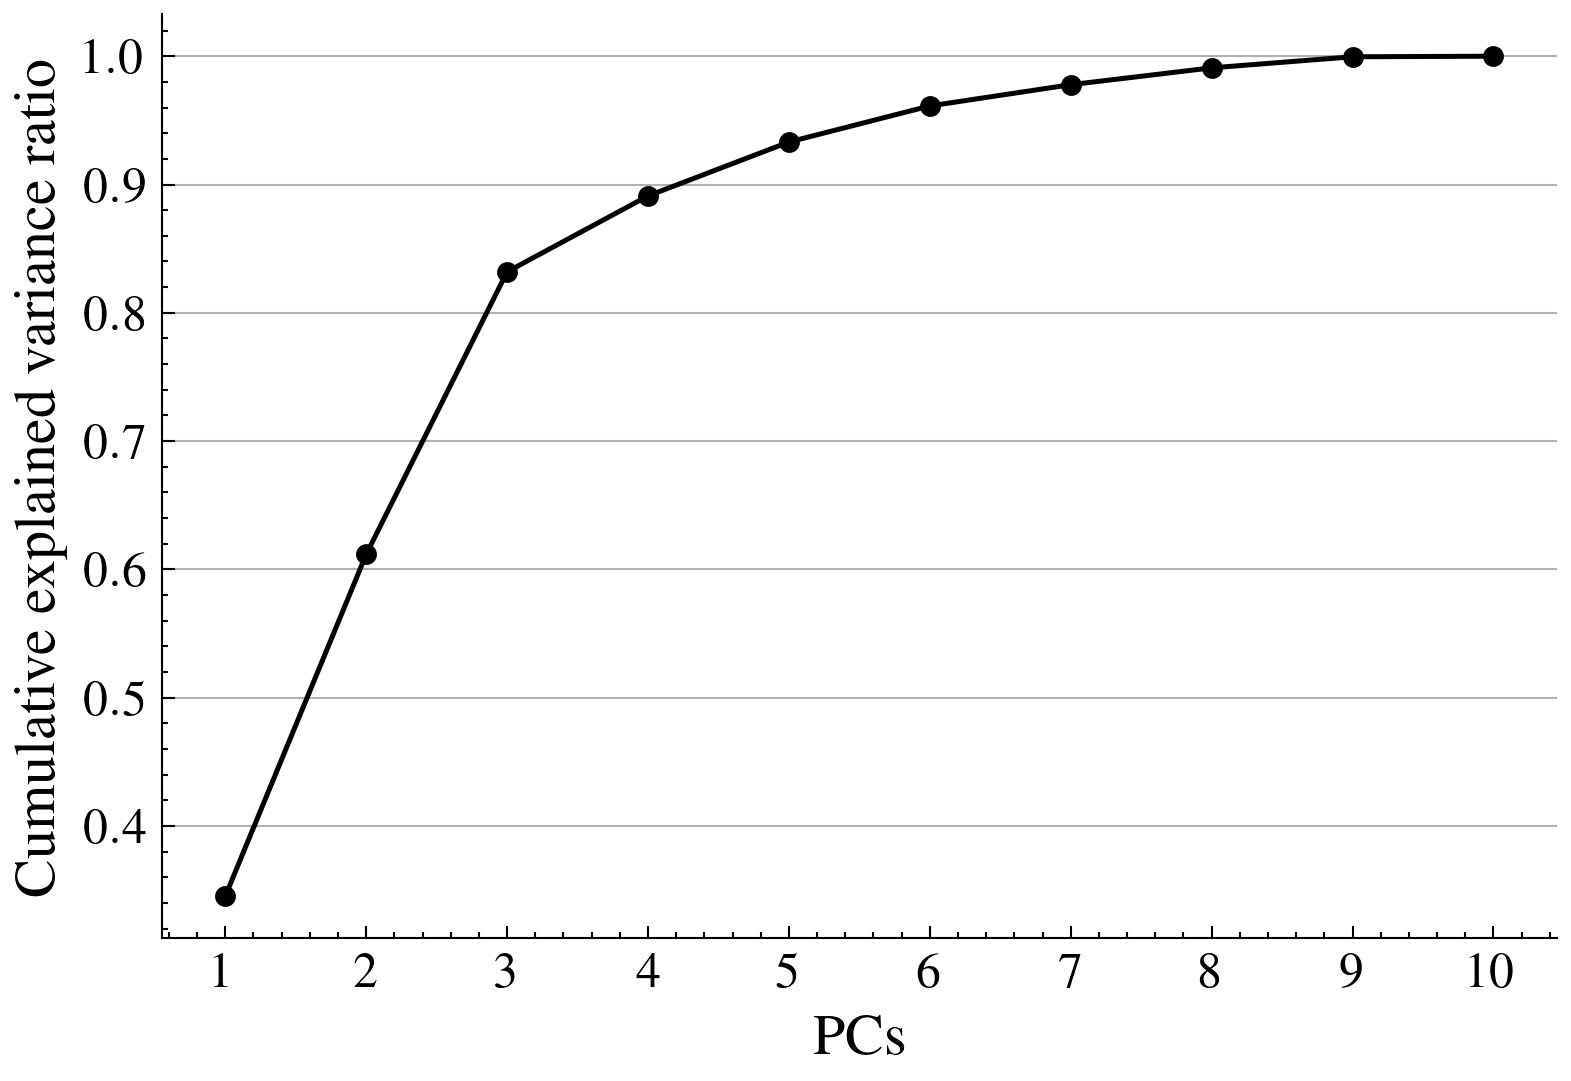
\includegraphics[width=\textwidth]{results/img/pca_explained_variance_ratio.png}
        \caption{}
        \label{fig:pca}
    \end{subfigure}
    \begin{subfigure}{0.49\textwidth}
        \centering
        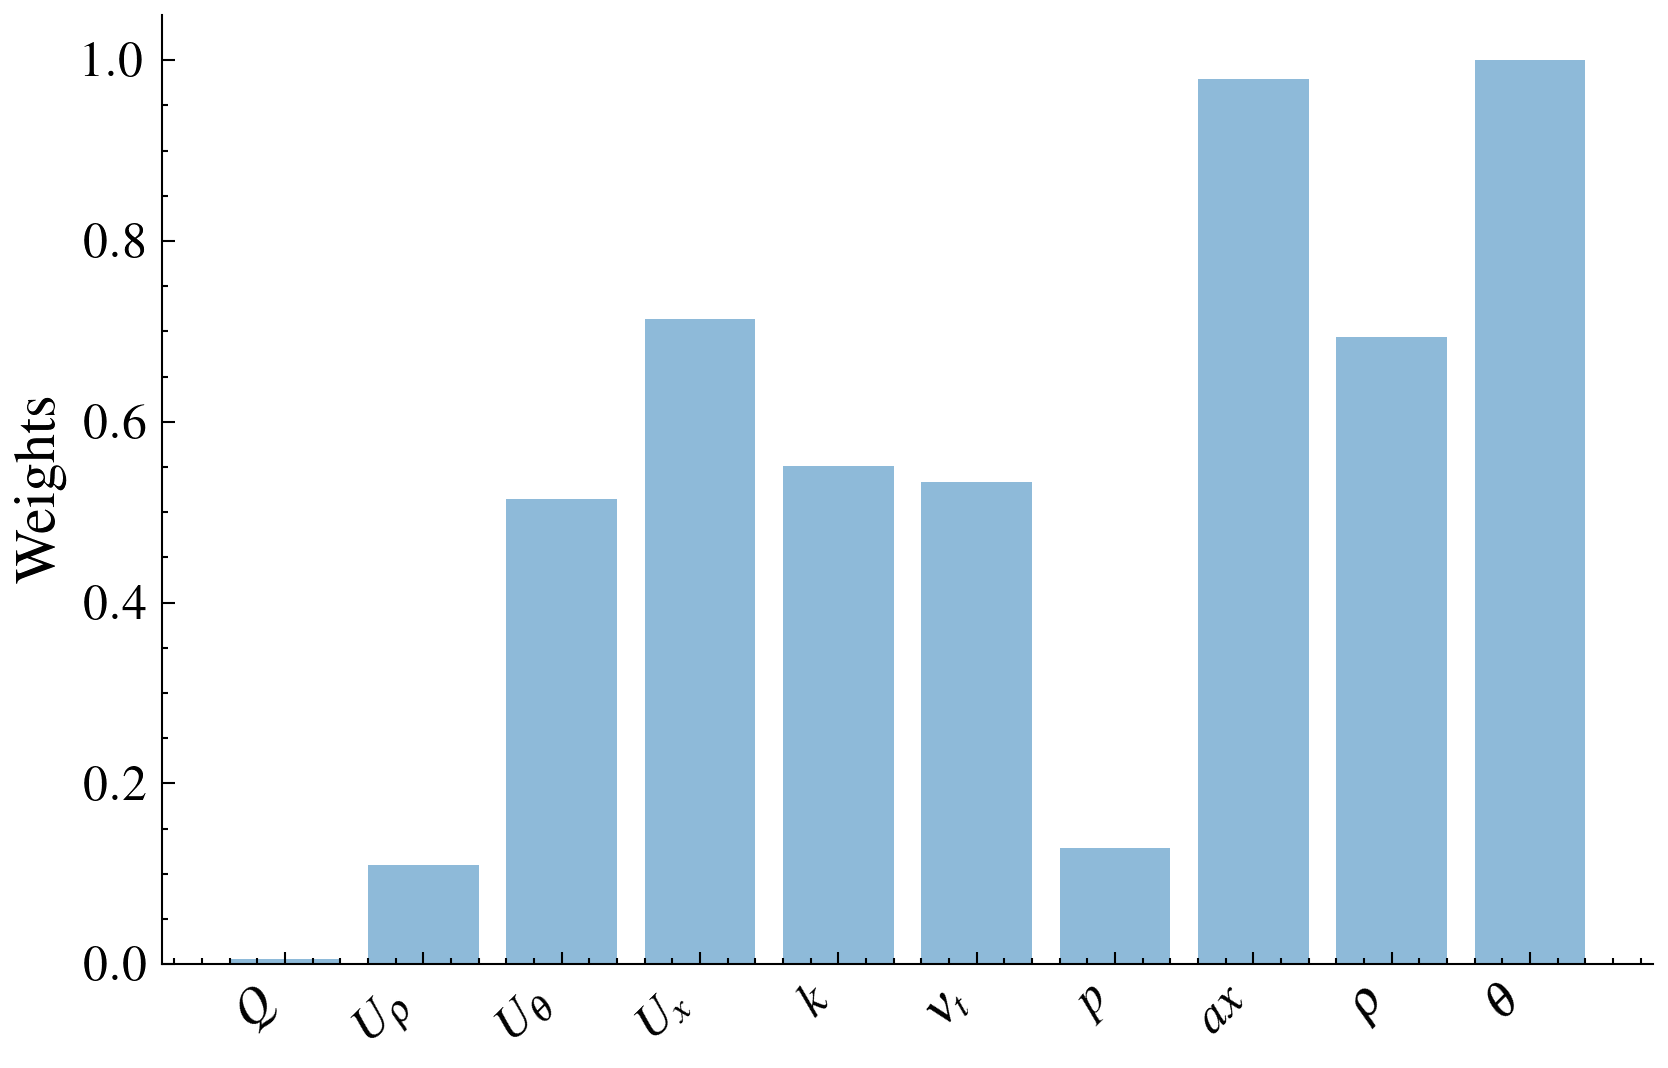
\includegraphics[width=\textwidth]{results/img/pca_features_weights.png}
        \caption{}
        \label{fig:pca_features_weights}
    \end{subfigure}
    \caption{PCA results: (a) explained variance ratio, (b) features weights on the first 6 PCA components.}
\end{figure}
From Fig.~\ref{fig:pca} it can be seen that the first 6 PCs explain more than 90\% of the variance. From Fig.~\ref{fig:pca_features_weights} the influence of the features on the first 6 PCs can be seen. It can be noted that the most influential features are the ones related to the cells coordinates (expressed in cylindrical coordinates) followed by $k$, $\nu_t$ and $U_x$.
$Q$ and $\mathbf{R}$ are not considered since they are inherently related to $\vec{U}_{cyl}$ and $k$ so they do not add any information to the clustering. This leads to the choice of $U_x$, $U_\theta$, $U_\rho$, $k$, $\nu_t$ and the cells coordinates as features for the clustering.
Since the spatial information is contained in the clusters, the cell-coordinate-related features are discarded. Moreover, since the clustering operations are performed in a pipeline in which the correction must affect the velocity field, both the $k$ and $\nu_t$ features are discarded since they are directly related to the correction to be predicted by the NN model, which is the eddy viscosity correction. Thus, only $U_x$, $U_\theta$ and $U_\rho$ are retained as features for the clustering.

The next step consists into determining the optimal number of clusters. The elbow chart for the clustering is shown in Fig.~\ref{fig:elbow_chart}. 
\begin{figure}[h]
    \centering
    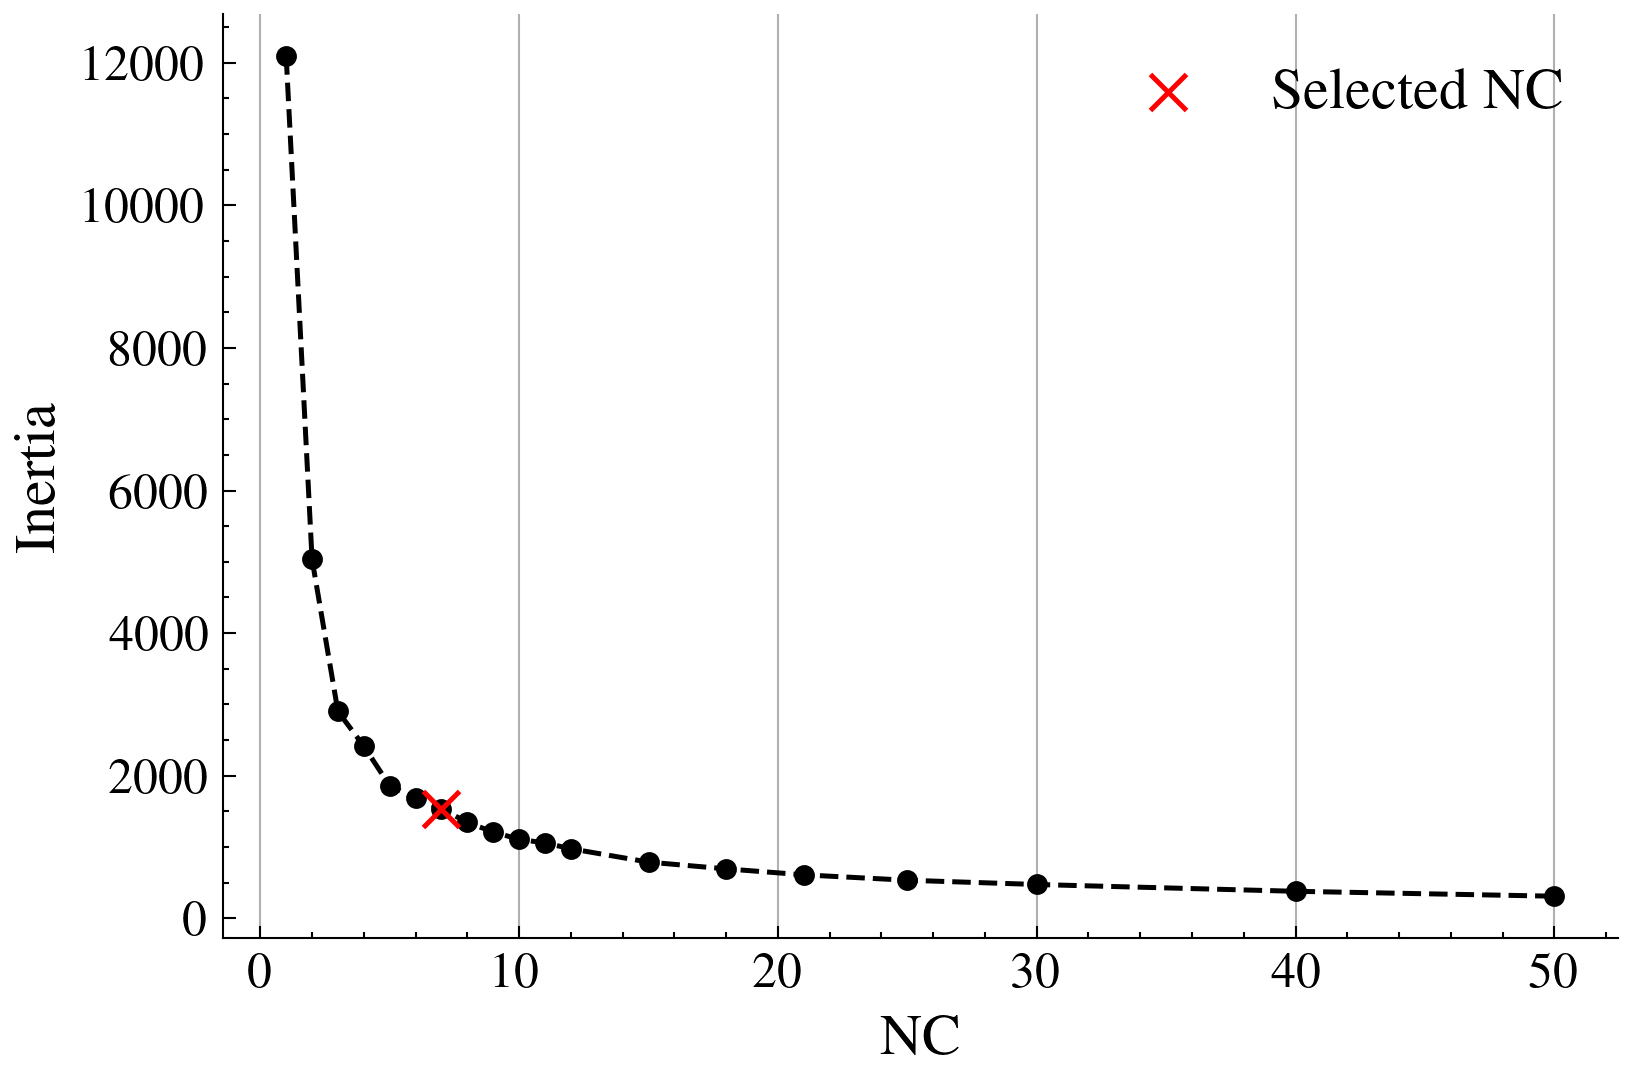
\includegraphics[width=0.6\textwidth]{results/img/elbow_plot.png}
    \caption{Elbow chart for the clustering.}
    \label{fig:elbow_chart}
\end{figure}
The plot shows a clear elbow near $K=7$, which is thus chosen as the optimal number of clusters.
Once all the parameters of the clustering are defined, the clustering is applied to the whole dataset and the results are shown in Fig.~\ref{fig:clustering_results_tot}.
\begin{figure}[h]
    \centering
    \begin{subfigure}{0.49\textwidth}
        \centering
        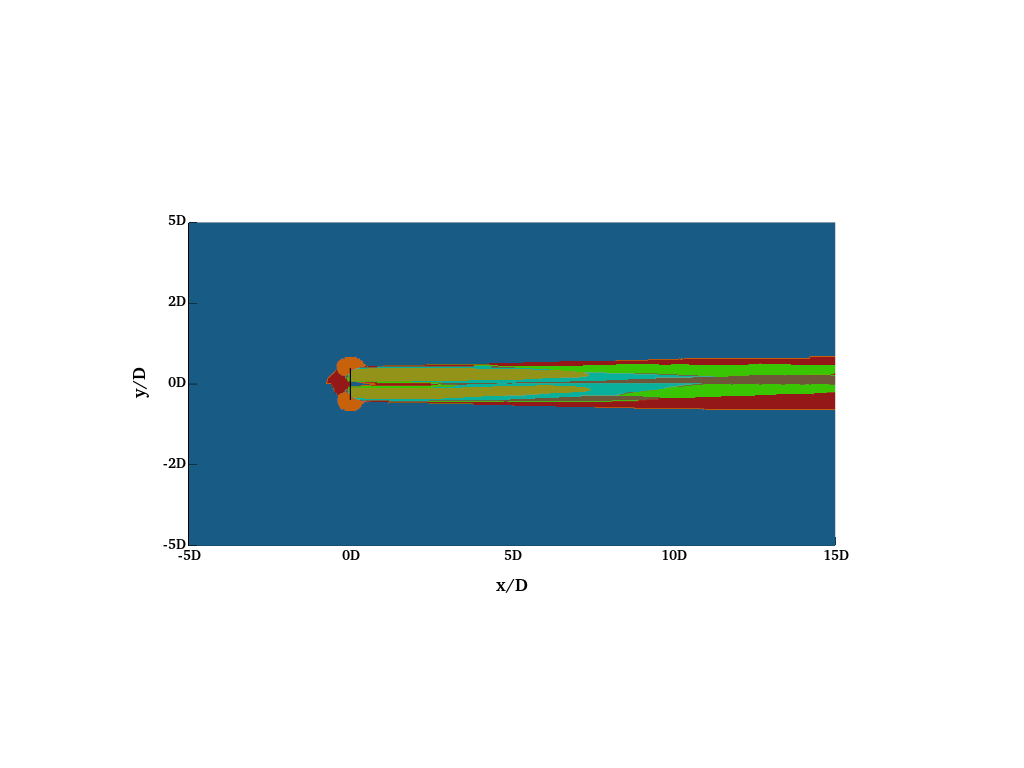
\includegraphics[width=\textwidth, trim=80 120 80 150, clip=true]{results/img/clustering_result_xy.png}
        \caption{}
        \label{fig:clustering_results}
    \end{subfigure}
    \hfill
    \begin{subfigure}{0.49\textwidth}
        \centering
        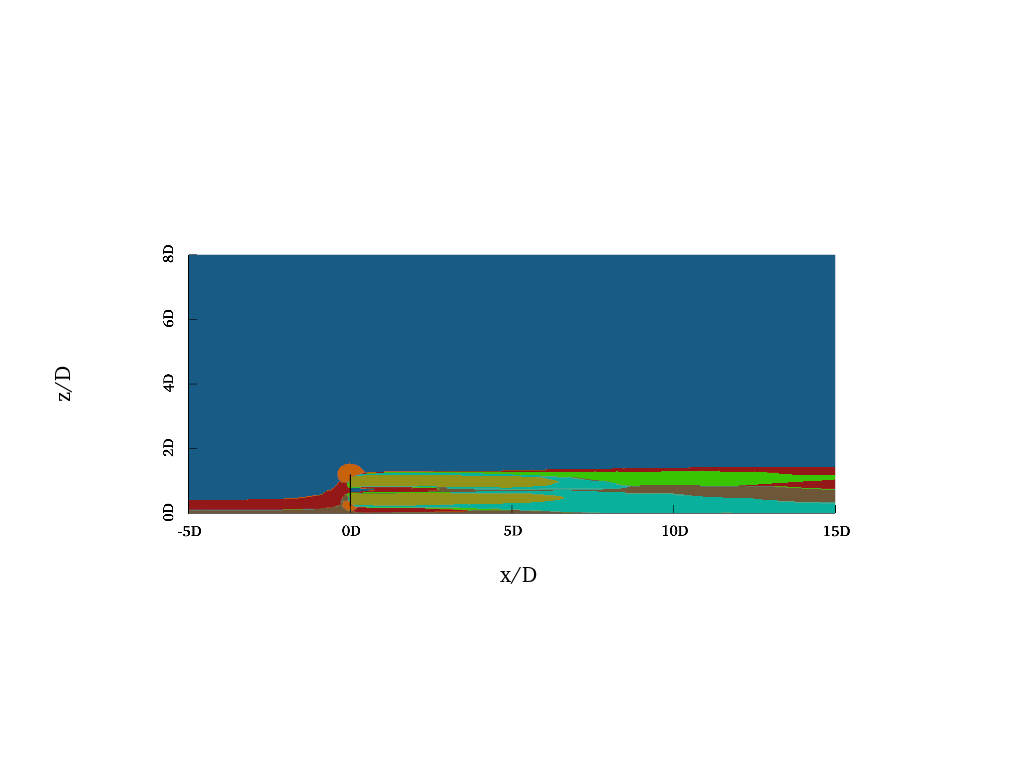
\includegraphics[width=\textwidth, trim=80 120 80 150, clip=true]{results/img/clustering_result_xz.png}
        \caption{}
        \label{fig:clustering_results_xz}
    \end{subfigure}
    \begin{subfigure}{0.6\textwidth}
        \centering
        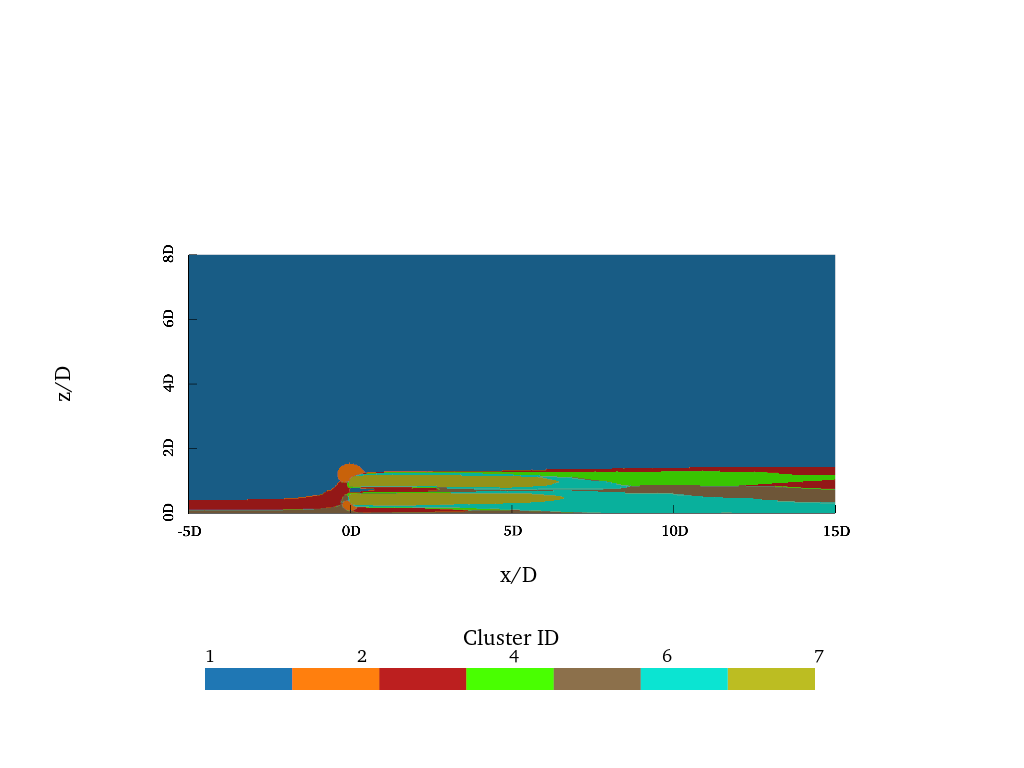
\includegraphics[width=\textwidth, trim=190 50 190 600, clip=true]{results/img/clustering_result_legend.png}
        \label{fig:clustering_results_legend}
    \end{subfigure}
    \caption{Clustering results: (a) xy view, (b) xz view.}
    \label{fig:clustering_results_tot}
\end{figure}
Different regions of the flow are clearly identified by the clustering. A clear separation between the disturbed and undisturbed flow can be seen:
\begin{itemize}
    \item Cluster 1 identifies the undisturbed flow.
    \item Clusters from 2 to 7 identify wake. In particular, cluster 3 identifies the inlet-ABL-affected region upstream of the rotor and the upper far-wake region; cluster 4 identifies the lower ABL-influenced far-wake region; the near-wake is identified by cluster 6, while cluster 5 highlights the near-wake region with higher $k$ levels and the mixing/breakdown region; finally, cluster 7 identifies the upstream rotor-inlet region.
\end{itemize}
Clusters validation is performed as in \cite{Carloni2026} and will not be shown here for brevity but the results are consistent with the reference and with the physical phenomena occurring in the flow. The clustering results are thus considered valid and the clusters are used for the training of the ML-based RANS model.
Clustering model is trained in $\sim 0.24$ seconds on the previously defined workstation and dataset.

\subsection{NN results}
\label{sec:NN_results}
The NN model is trained using the fixed manual configuration described in Sec.~\ref{sec:ML_part}.

The network predicts the standardised correction $\Delta \nu_t=\nu_{t,eq}-\nu_{t,\mathrm{RANS}}$ and the final eddy viscosity is reconstructed as $\nu_{t,ML}=\nu_{t,\mathrm{RANS}}+\Delta \nu_{t,ML}$. In the reported run, trained on the $U_\infty=11\,\mathrm{m/s}$ operating condition, the best checkpoint is obtained at epoch 220, where $validation\ loss=2.47\cdot10^{-2}$ and $validation\ MAE=2.86\cdot10^{-2}$ in normalized target space. On the training set the reconstructed physical field reaches $R^2=0.9954$, $RMSE=0.2584$ and $MAE=0.1769$, while the validation subset gives $R^2=0.9952$, $RMSE=0.2635$ and $MAE=0.1797$.

The training and validation loss curves are shown in Fig.~\ref{fig:training_curves} as also the scatter plot of the predicted and true $\nu_t$ values on the test set.
\begin{figure}
    \centering
    \begin{subfigure}{0.32\textwidth}
        \centering
        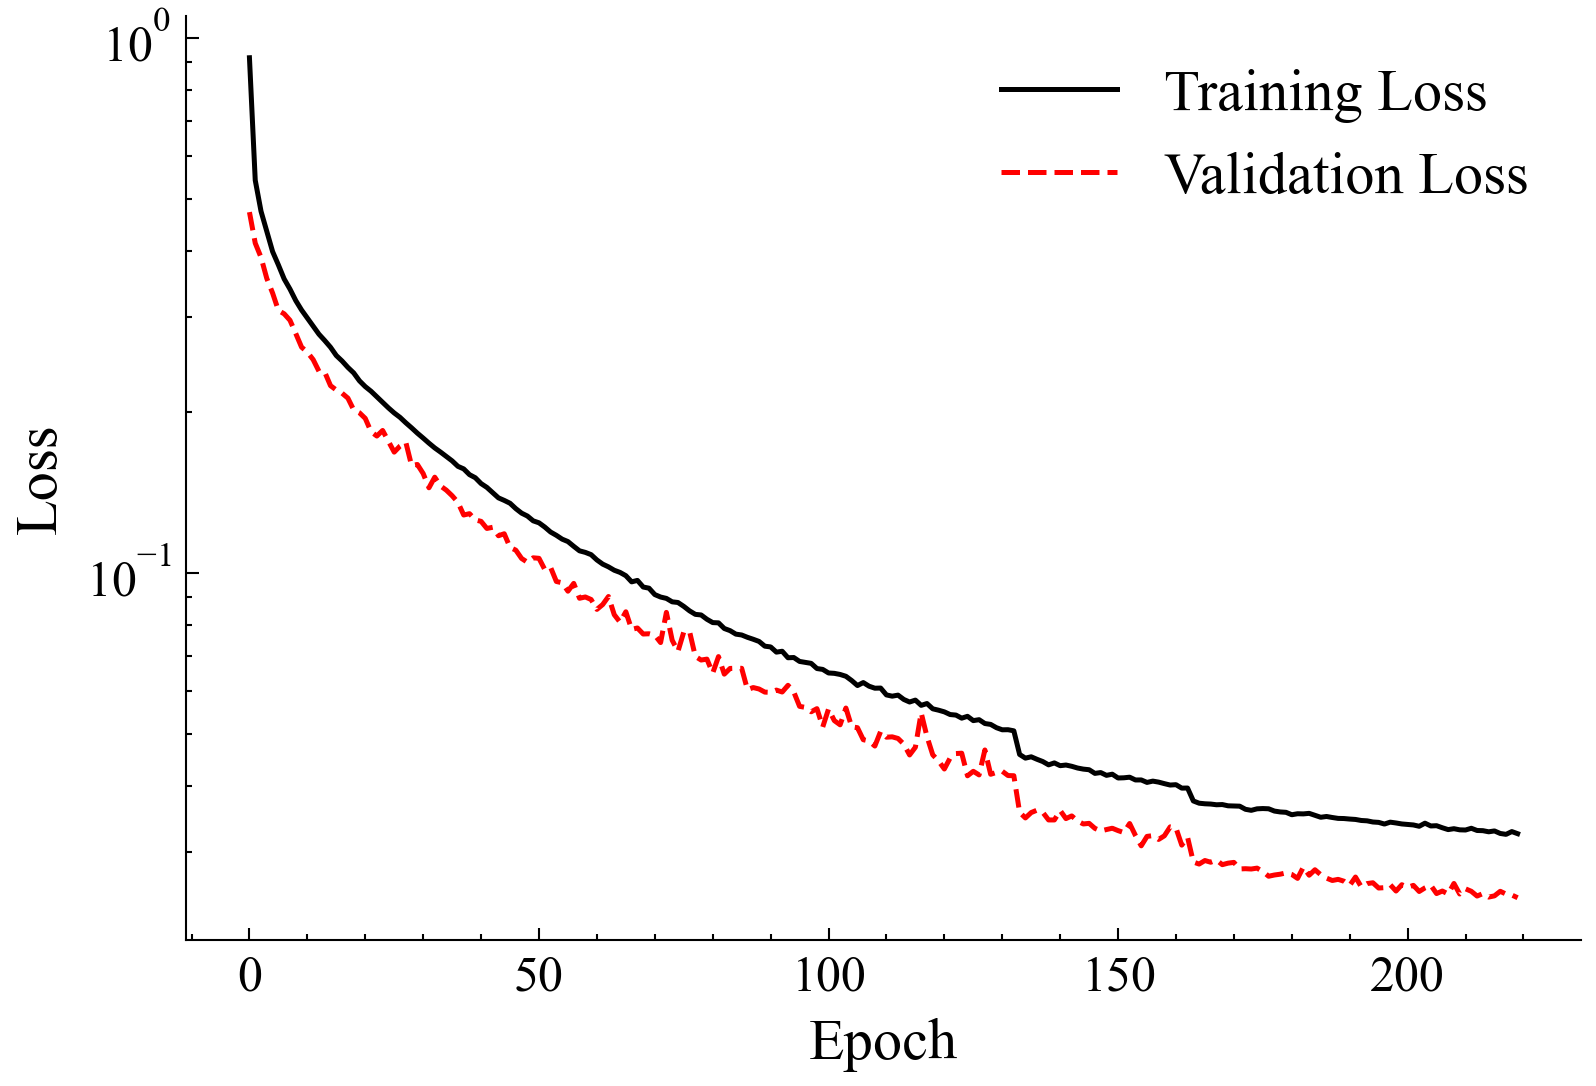
\includegraphics[width=\textwidth]{results/img/NN_loss_curves.png}
        \caption{}
        \label{fig:NN_loss_curves}
    \end{subfigure}
    \hfill
    \begin{subfigure}{0.32\textwidth}
        \centering
        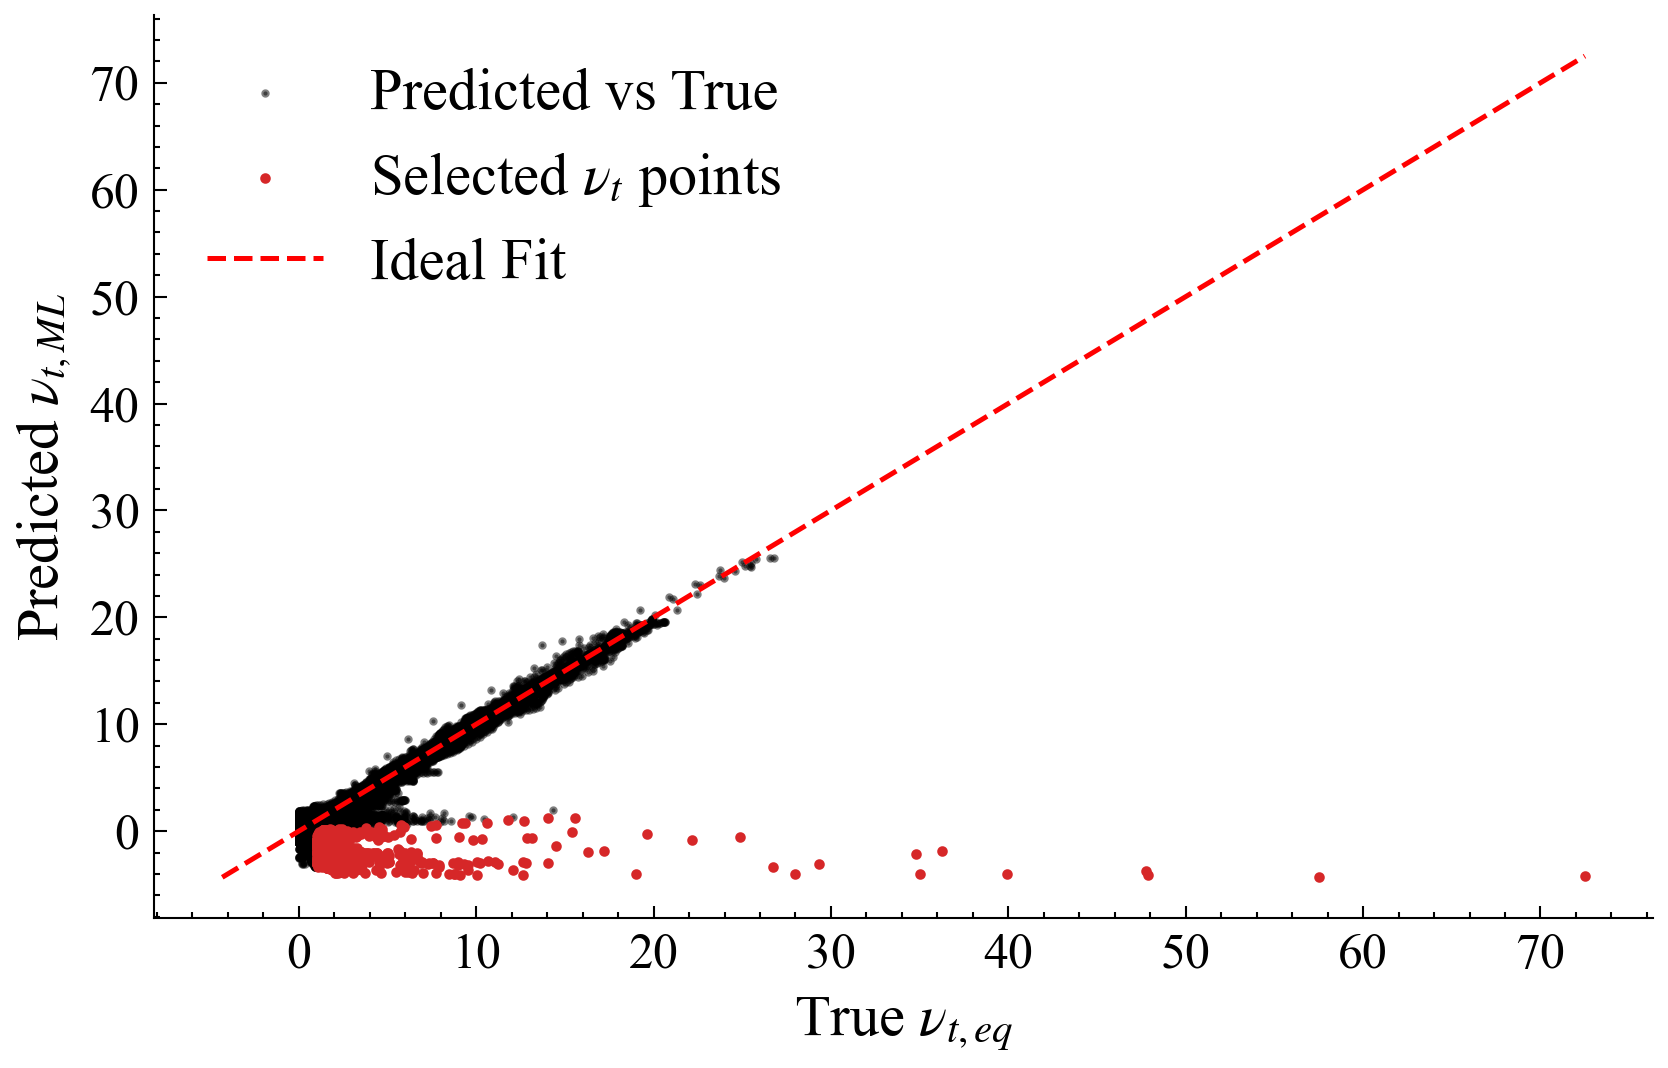
\includegraphics[width=\textwidth]{results/img/ml_results/bias_points/nut_scatter_bias_points_highlighted.png}
        \caption{}
        \label{fig:NN_scatter_plot}
    \end{subfigure}
    \hfill
    \begin{subfigure}{0.32\textwidth}
        \centering
        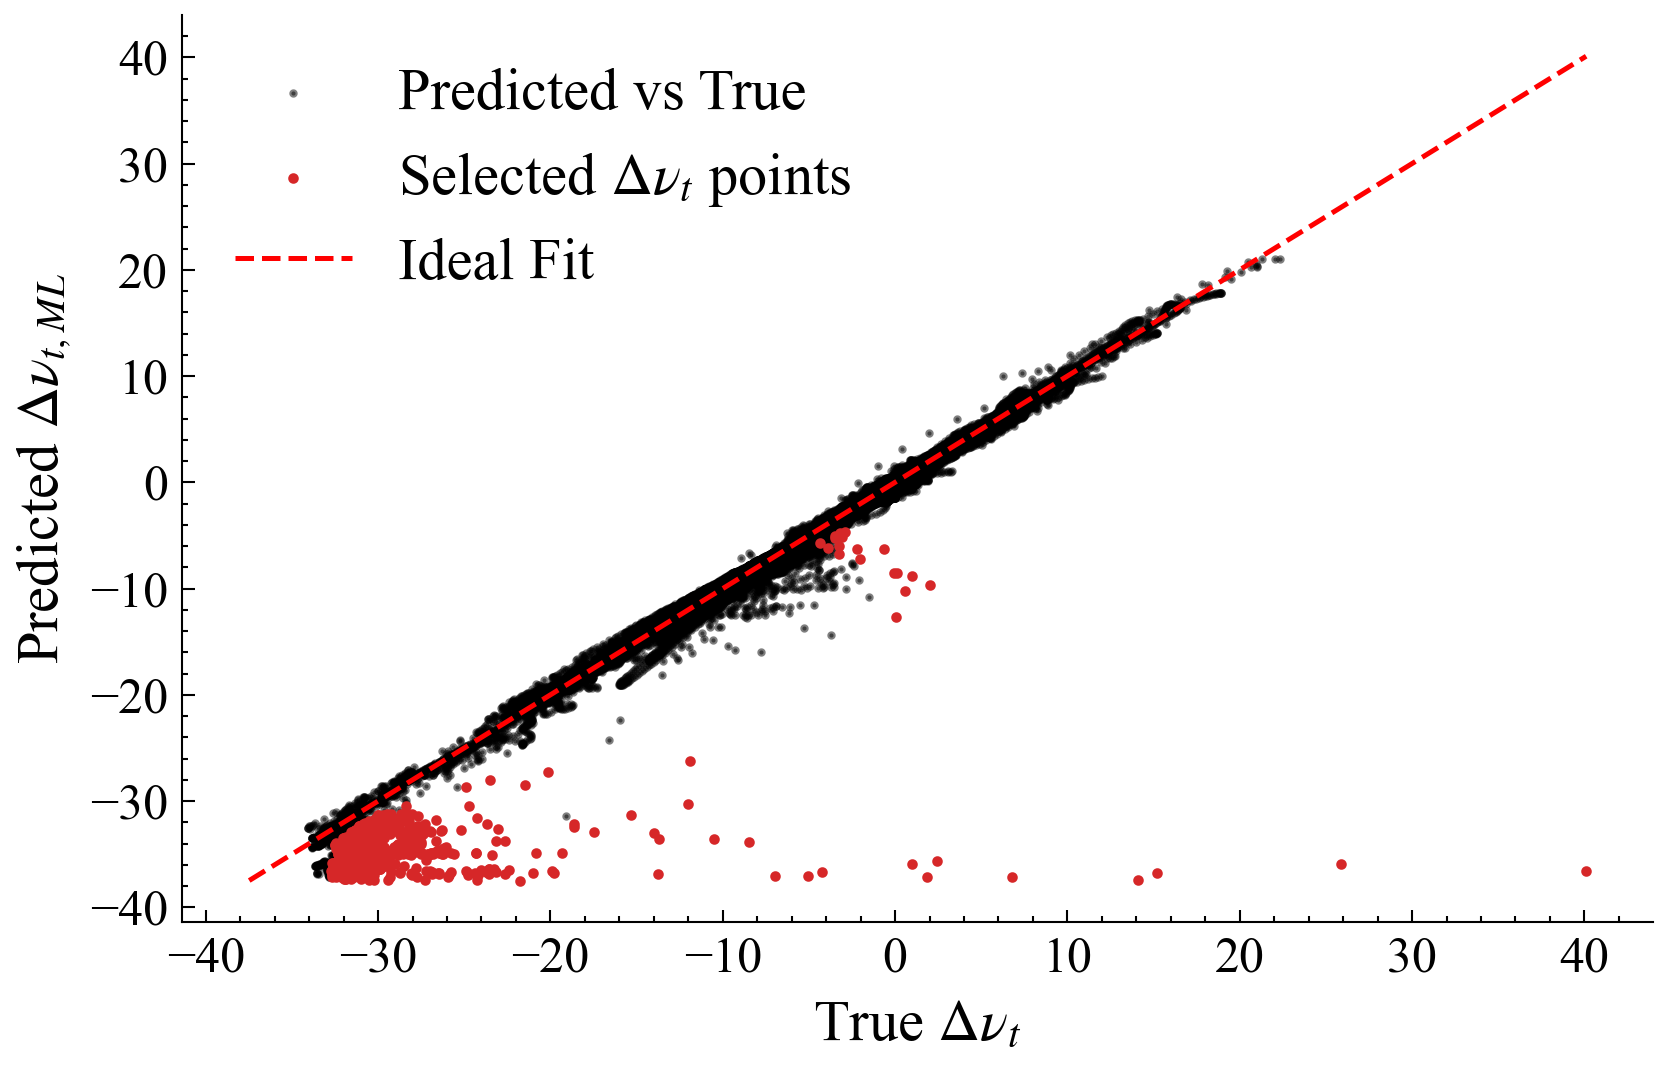
\includegraphics[width=\textwidth]{results/img/ml_results/bias_points/delta_scatter_bias_points_highlighted.png}
        \caption{}
        \label{fig:NN_delta_scatter_plot}
    \end{subfigure}
    \begin{subfigure}{0.5\textwidth}
        \centering
        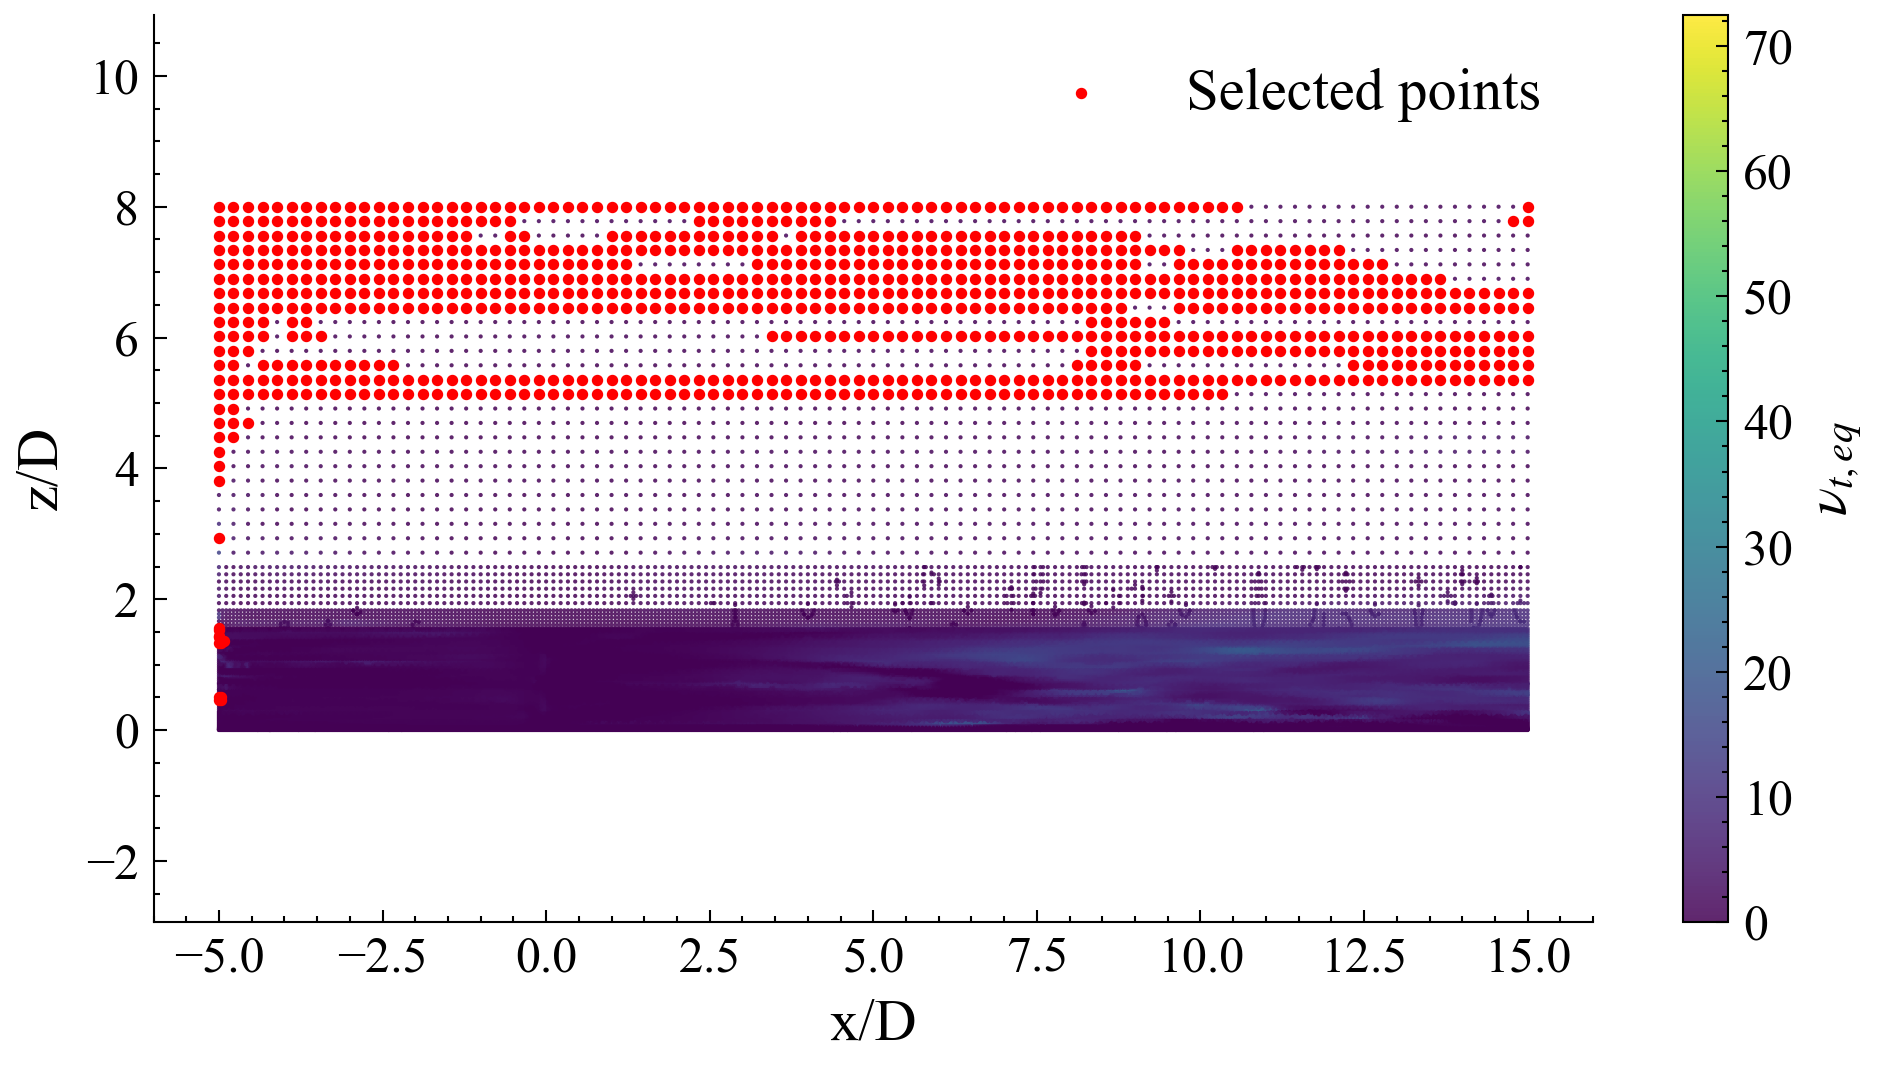
\includegraphics[width=\textwidth]{results/img/ml_results/bias_points/delta_bias_points_on_y0_slice.png}
        \caption{}
        \label{fig:NN_scatter_plot_legend}        
    \end{subfigure}
    \caption{NN results: (a) training and validation loss curves, (b) scatter plot of predicted vs true $\nu_t$ values on the test set, (c) scatter plot of predicted vs true $\Delta \nu_t$ values on the test set, (d) slice plot of selected high-error points.}
    \label{fig:training_curves}
\end{figure}
From Fig.~\ref{fig:NN_loss_curves} a small gap between the training and validation loss can be observed, consistent with the deliberately compact training set, which by design consists of a single operating condition ($U_\infty=11\,\mathrm{m/s}$) sampled on a single grid. This gap is the expected price of the single-case calibration that is central to the methodology, and it does not compromise the predictive use of the closure: the two curves do not diverge, the validation metrics are essentially identical to the training ones ($R^2=0.995$ in both), and, as shown in Sec.~\ref{sec:generalization}, the embedded model transfers accurately to grids and inflow velocities outside the training set. Accordingly, the NN predictions are accurate, as shown in Fig.~\ref{fig:NN_scatter_plot}, where the predicted $\Delta \nu_{t,ML}$ values are close to the true $\Delta \nu_{t}$ values, as also happens in Fig.~\ref{fig:NN_delta_scatter_plot}, where the predicted $\nu_{t,ML}$ values are close to the true $\nu_{t,eq}$ values. A series of outliers can be noted in the predictions, in the marked region of the scatter plots, where the NN underestimates the true $\nu_{t,eq}$ values. This is inherited from the same bias area highlighted in the scatter plot of the $\Delta \nu_{t,ML}$ values, where the NN underestimates the true $\Delta \nu_t$ values. This, as Fig.~\ref{fig:NN_scatter_plot_legend} shows, corresponds to a specific region of the domain, located at the inlet, in which numerical instabilities are present due to the coded inlet boundary condition. In such area the NN predictions are less accurate, but this is not expected to significantly affect the overall performance of the ML-based RANS model.
In fact, the NN predictions are still accurate and the NN-based RANS model is expected to perform better than the standard RANS model, as shown in the next section. The resulting $\nu_{t,ML}$ field is shown in Fig.~\ref{fig:nu_t_fields} together with the $\nu_{t,eq}$ and $\nu_{t,\mathrm{RANS}}$ fields for comparison.
\begin{figure}
    \centering
    \begin{subfigure}{0.32\textwidth}
        \centering
        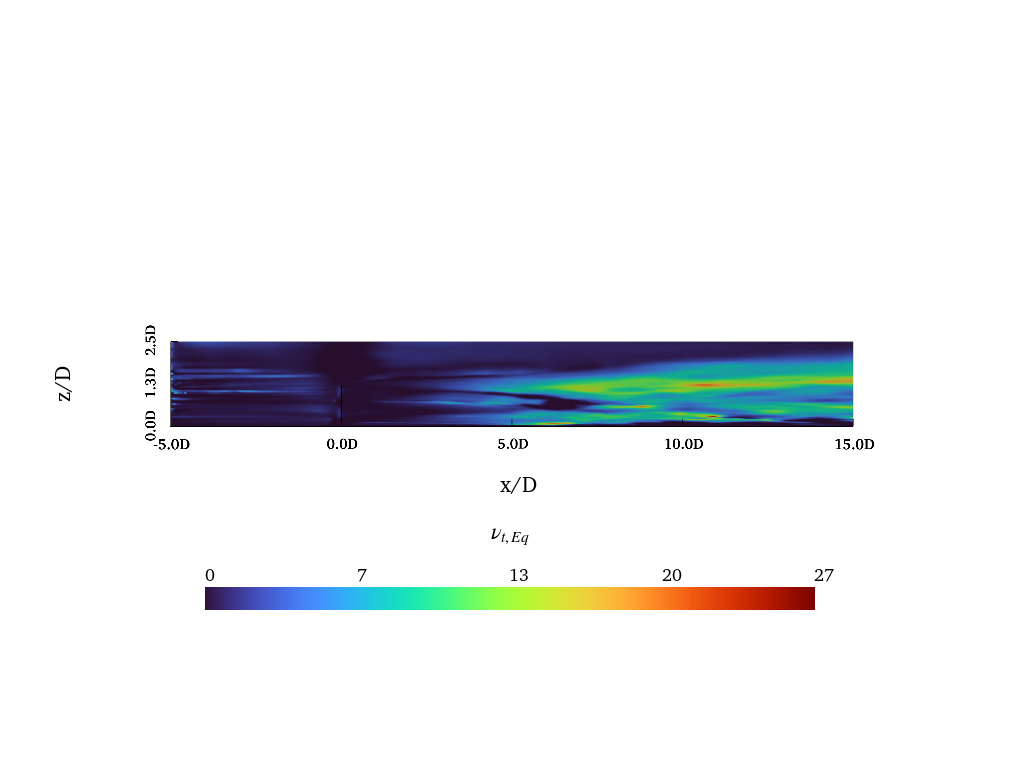
\includegraphics[width=\textwidth, trim=80 120 80 150, clip=true]{results/img/nutEq_field_xz.png}
        \caption{}
        \label{fig:nu_t_eq}
    \end{subfigure}
    \hfill
    \begin{subfigure}{0.32\textwidth}
        \centering
        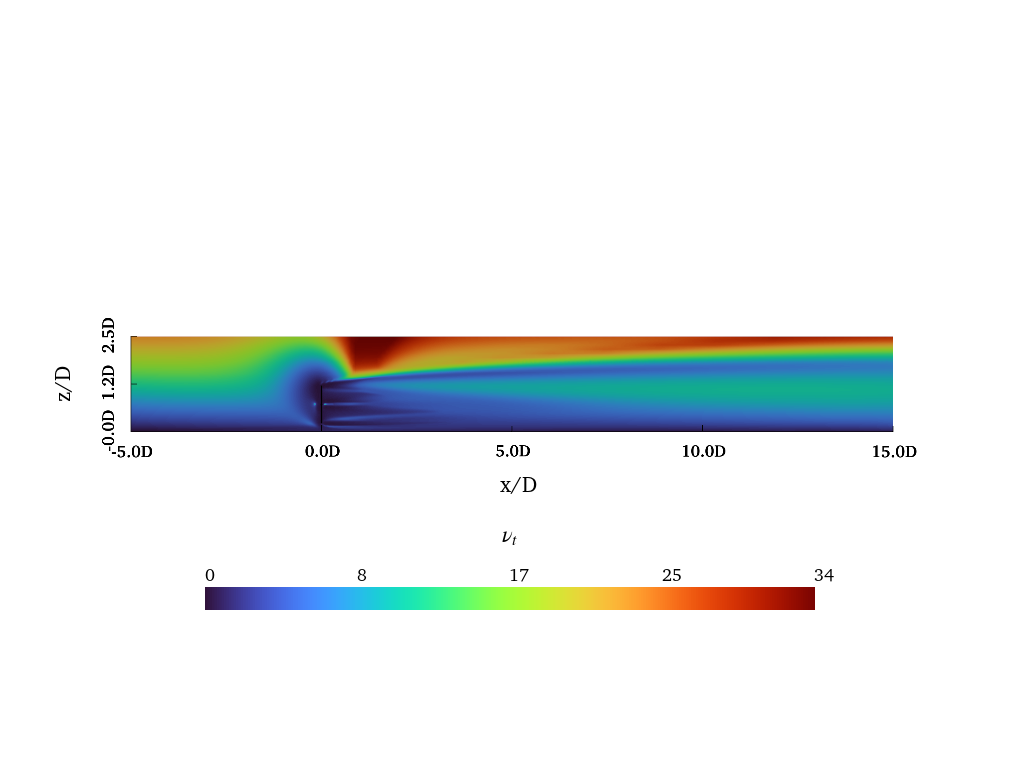
\includegraphics[width=\textwidth, trim=80 120 80 150, clip=true]{results/img/nut_rans_field_xz.png}
        \caption{}
        \label{fig:nu_t_RANS}
    \end{subfigure}
    \hfill
    \begin{subfigure}{0.32\textwidth}
        \centering
        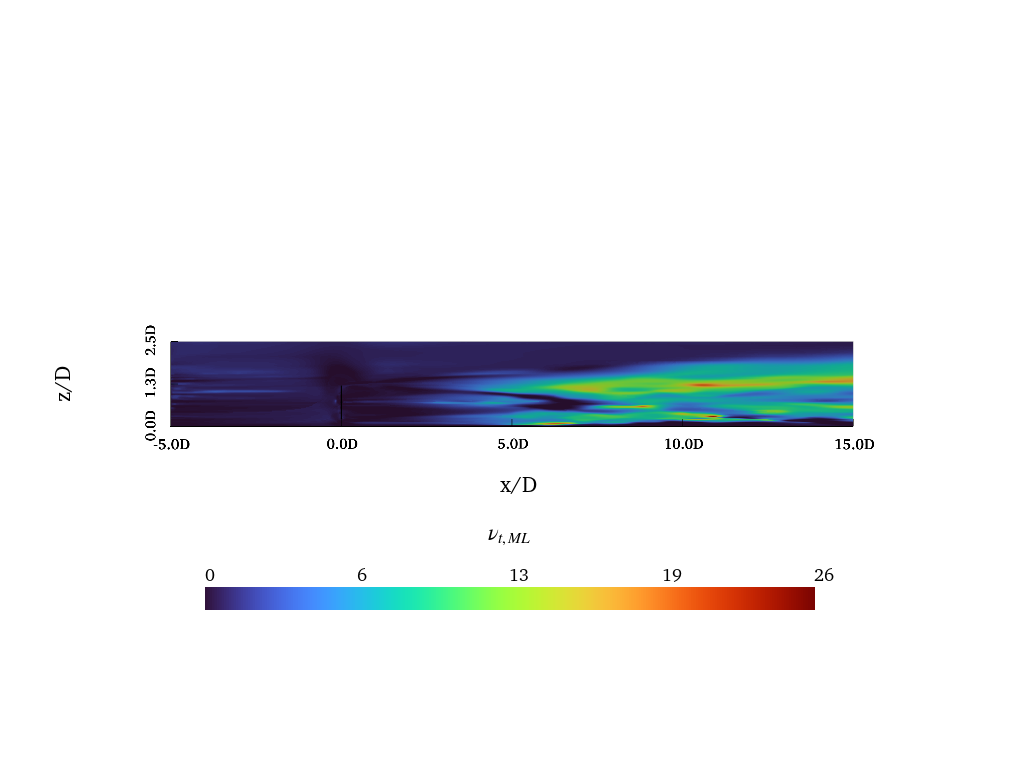
\includegraphics[width=\textwidth, trim=80 120 80 150, clip=true]{results/img/nut_pred_field_xz.png}
        \caption{}
        \label{fig:nu_t_ML}
    \end{subfigure}
    \caption{Eddy viscosity fields: (a) $\nu_{t,eq}$, (b) $\nu_{t,\mathrm{RANS}}$ (obtained by importing the mean pressure and velocity field of the LES in the RANS solver), (c) $\nu_{t,ML}$.}
    \label{fig:nu_t_fields}
\end{figure}

\subsection{ML-based RANS model results}
\label{sec:ml_rans_results}
The trained ML model is embedded in the RANS solver as described in Sec.~\ref{sec:ML_part} and evaluated across grids of different resolutions to assess both its predictive accuracy and its computational efficiency.

To highlight the importance of clustering in the methodology, the ML-based RANS model was compared against a variant trained without clustering, using the same network architecture and hyperparameters without all clustering-related components. The best validation loss for the unclustered model is obtained at epoch 219, with $validation\ loss \approx 2.44\cdot10^{-2}$ and $validation\ MAE = 2.95\cdot10^{-2}$ in the normalised target space. On the validation subset, the reconstructed physical field reaches $R^2 = 0.9950$, $RMSE = 0.2713$ and $MAE = 0.1812$. All these metrics are slightly worse than in the clustered case ($R^2 = 0.9952$, $RMSE = 0.2635$, $MAE = 0.1797$), indicating that clustering allows the model to better capture the variance of the data and thus to reconstruct the physical field more faithfully. The aggregate metrics differ only marginally because they are dominated by the large, well-behaved free-stream region; the value of clustering, however, lies not in the global score but in \emph{where} the improvement is concentrated, in its robustness to mesh refinement and in the physical interpretability it provides, as discussed in the following. The training and validation loss curves together with the scatter plots of the predicted and true $\nu_t$ and $\Delta \nu_t$ values on the test set are shown in Fig.~\ref{fig:training_curves_no_clustering}.

\begin{figure}
    \centering
    \begin{subfigure}{0.32\textwidth}
        \centering
        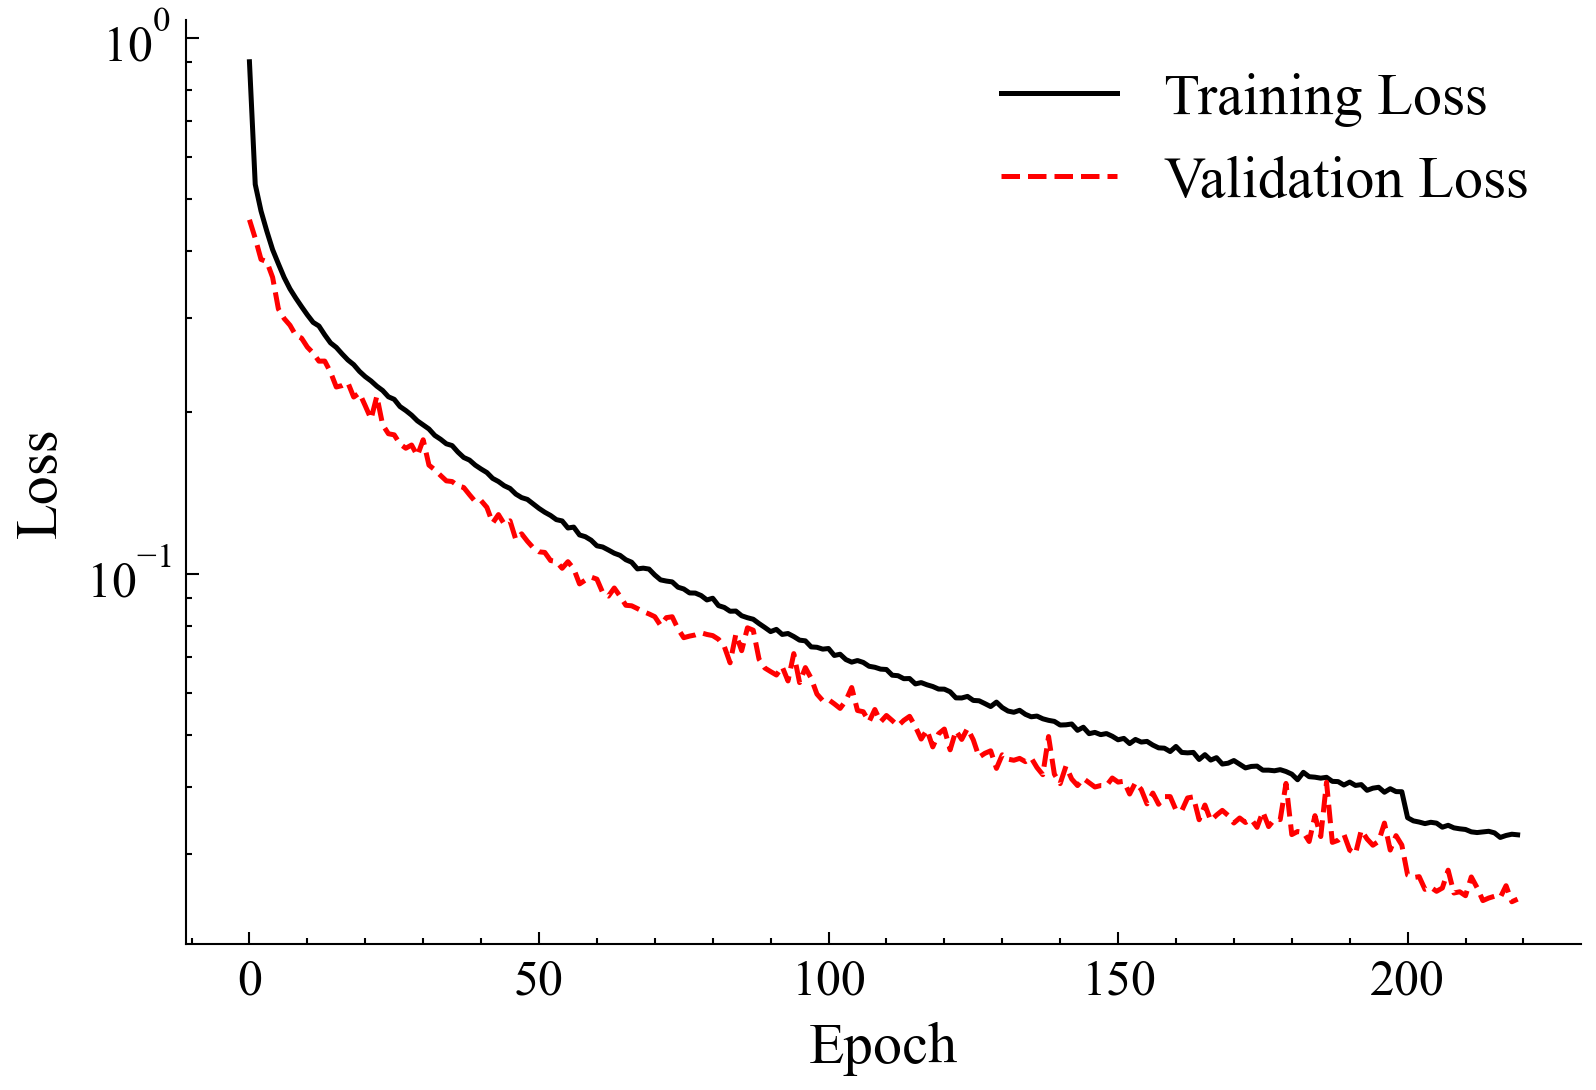
\includegraphics[width=\textwidth]{results/img/NN_loss_curves_no_clustering.png}
        \caption{}
        \label{fig:NN_loss_curves_no_clustering}
    \end{subfigure}
    \hfill
    \begin{subfigure}{0.32\textwidth}
        \centering
        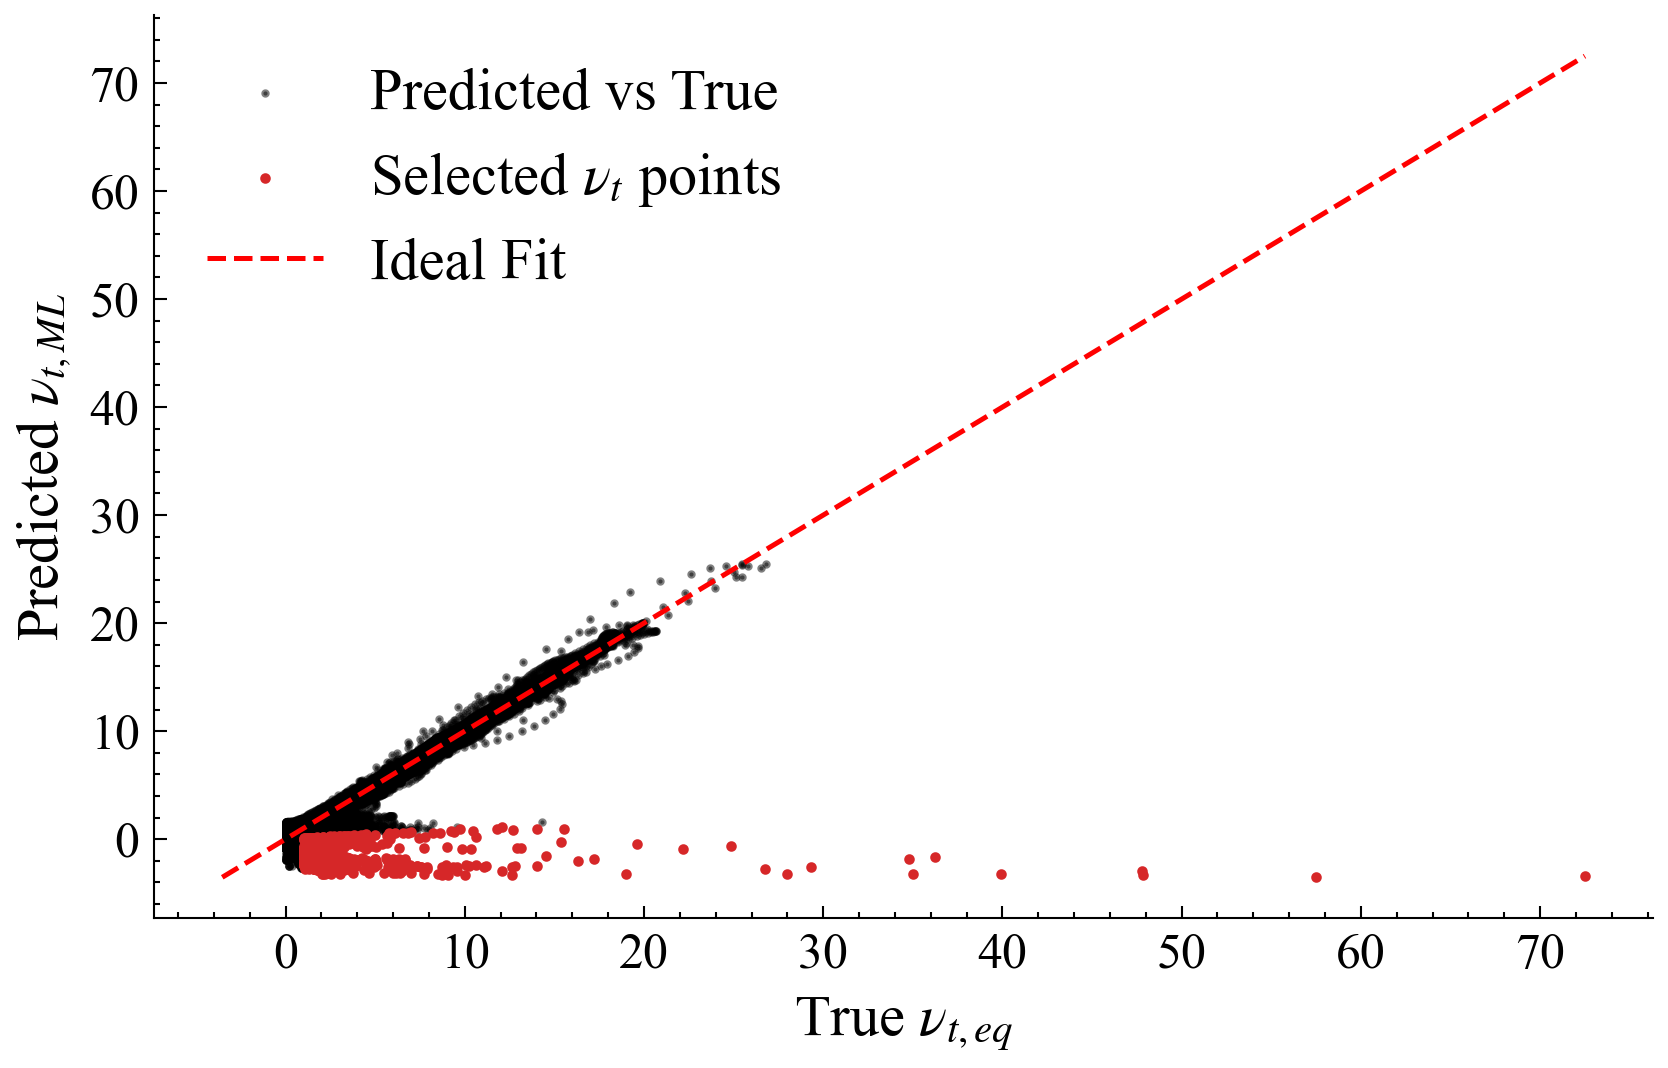
\includegraphics[width=\textwidth]{results/img/ml_results/bias_points/nut_scatter_bias_points_highlighted_no_clustering.png}
        \caption{}
        \label{fig:NN_scatter_plot_no_clustering}
    \end{subfigure}
    \hfill
    \begin{subfigure}{0.32\textwidth}
        \centering
        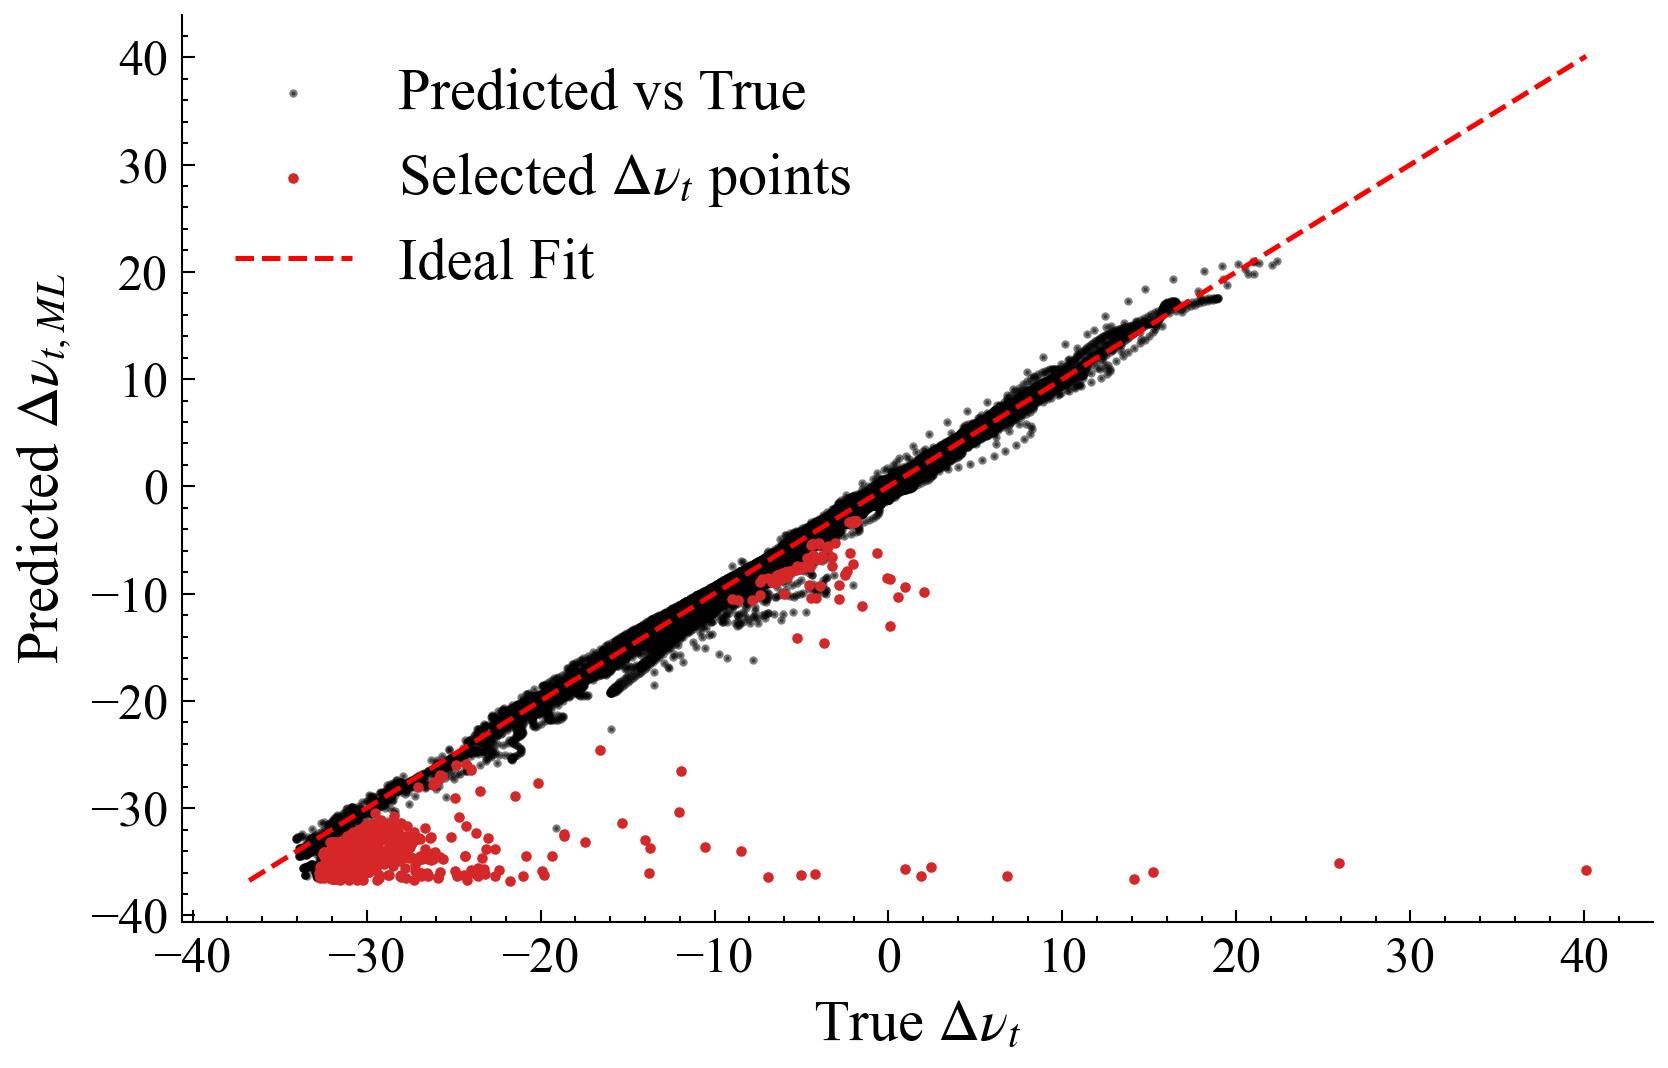
\includegraphics[width=\textwidth]{results/img/ml_results/bias_points/delta_scatter_bias_points_highlighted_no_clustering.png}
        \caption{}
        \label{fig:NN_delta_scatter_plot_no_clustering}
    \end{subfigure}
    \begin{subfigure}{0.5\textwidth}
        \centering
        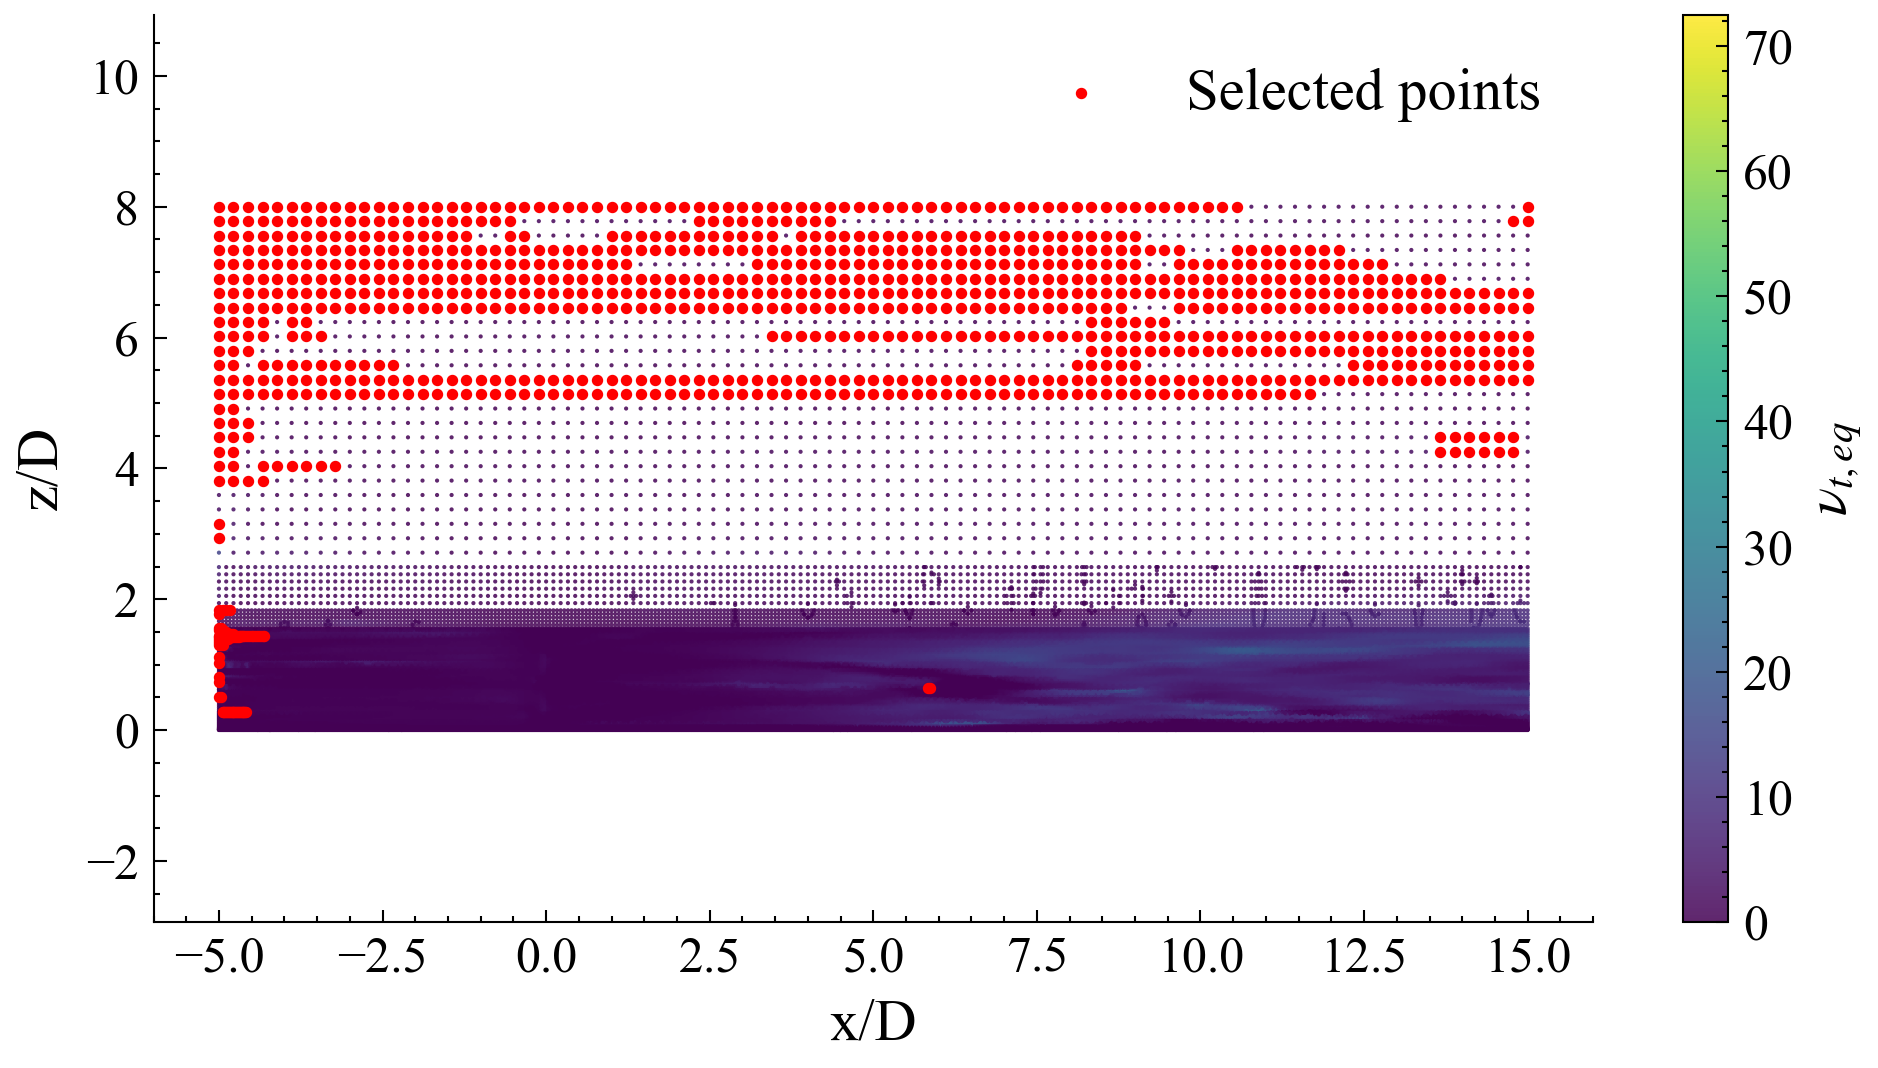
\includegraphics[width=\textwidth]{results/img/ml_results/bias_points/delta_bias_points_on_y0_slice_no_clustering.png}
        \caption{}
        \label{fig:NN_scatter_plot_legend_no_clustering}        
    \end{subfigure}
    \caption{NN results of the model without clustering: (a) training and validation loss curves, (b) scatter plot of predicted vs true $\nu_t$ values on the test set, (c) scatter plot of predicted vs true $\Delta \nu_t$ values on the test set, (d) slice plot of selected high-error points.}
    \label{fig:training_curves_no_clustering}
\end{figure}

As visible in Figures \ref{fig:NN_scatter_plot_no_clustering} and \ref{fig:NN_delta_scatter_plot_no_clustering}, the unclustered model exhibits the same underestimation bias in the inlet region as well as a slightly overfitting trend. More importantly, the absence of clustering leads to a degraded prediction in the near-terrain region, where the flow is strongly influenced by the ground boundary layer and exhibits high spatial variability. In this zone the clustered model produces results that are considerably more consistent with the LES reference, since clustering enables the network to learn separately the distinct flow regimes present in the near-wall and free-stream regions, rather than approximating them with a single global mapping.

Finally, the ML-based RANS model results are shown in Fig.~\ref{fig:ml_results}.

\begin{figure}
    \centering
    \begin{subfigure}{\textwidth}
        \centering
        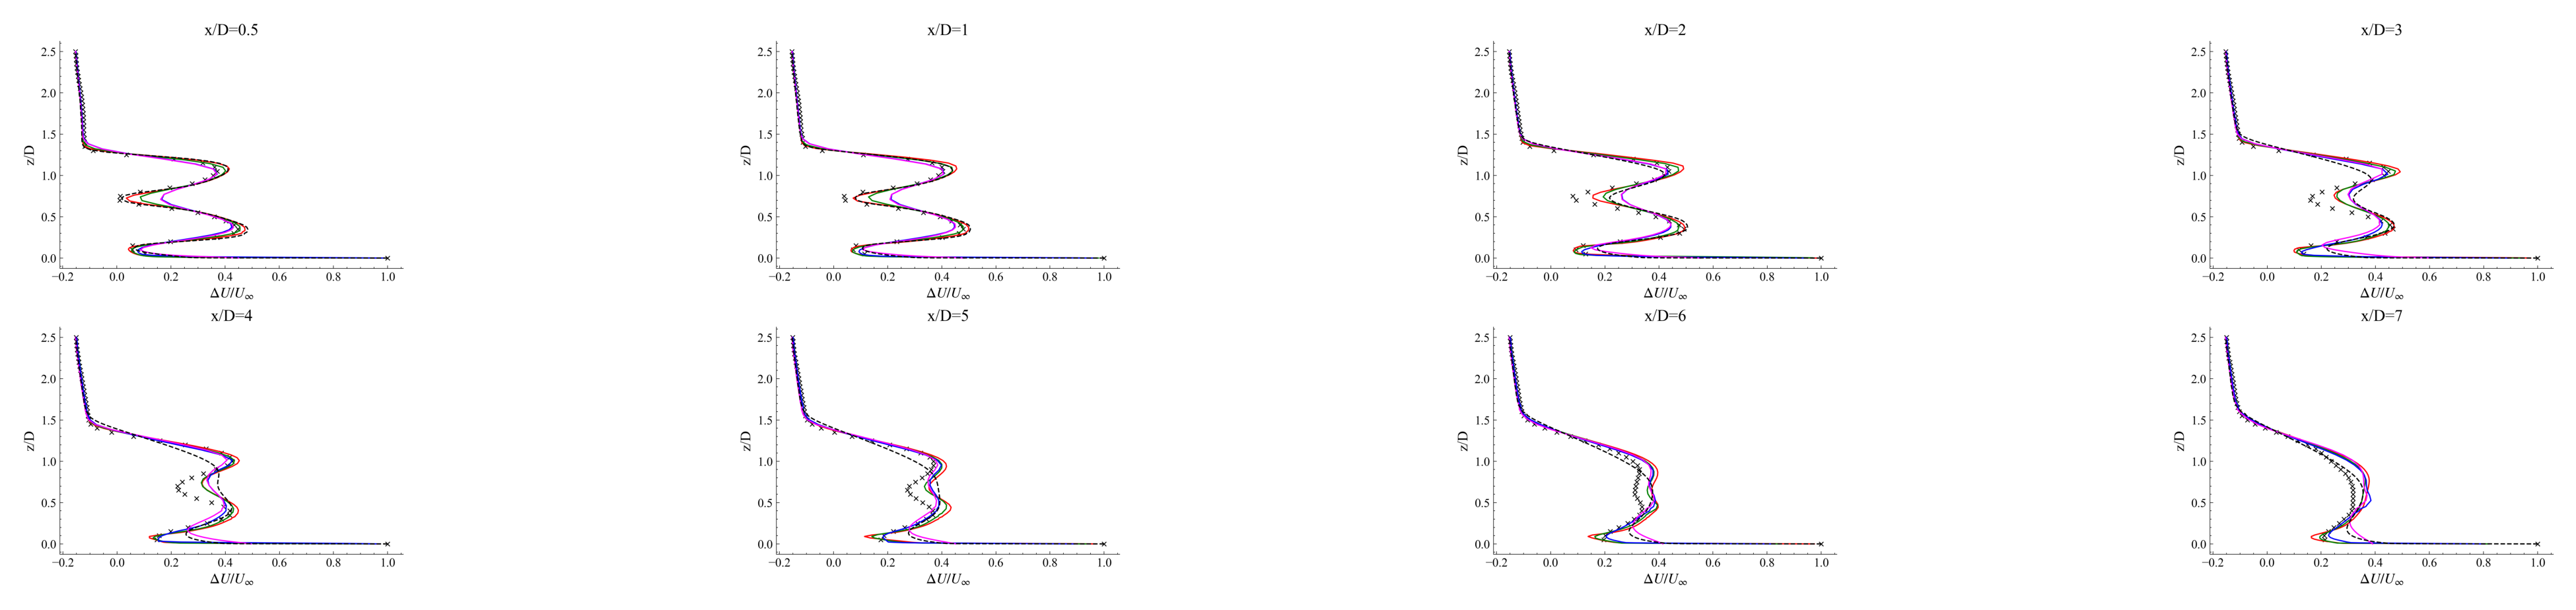
\includegraphics[width=\textwidth]{results/img/ml_results/11ms/deficit/ml_models_comparison/velocity/comparison.png}
        \caption{}
        \label{Fig:velocity_deficit}        
    \end{subfigure}
    \begin{subfigure}{0.3\textwidth}
        \centering
            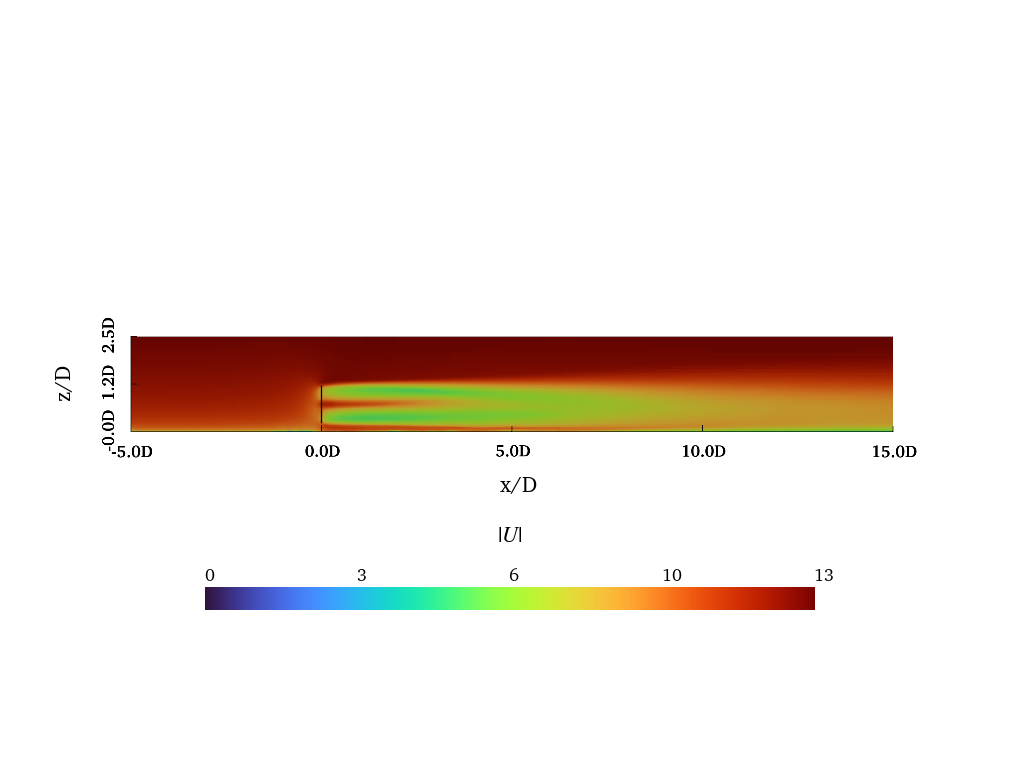
\includegraphics[width=\textwidth, trim=80 120 80 150, clip=true]{results/img/predicted_U_field_xz.png}
            \caption{}
        \label{Fig:velocity_plot}
    \end{subfigure}
    \begin{subfigure}{0.3\textwidth}
        \centering
        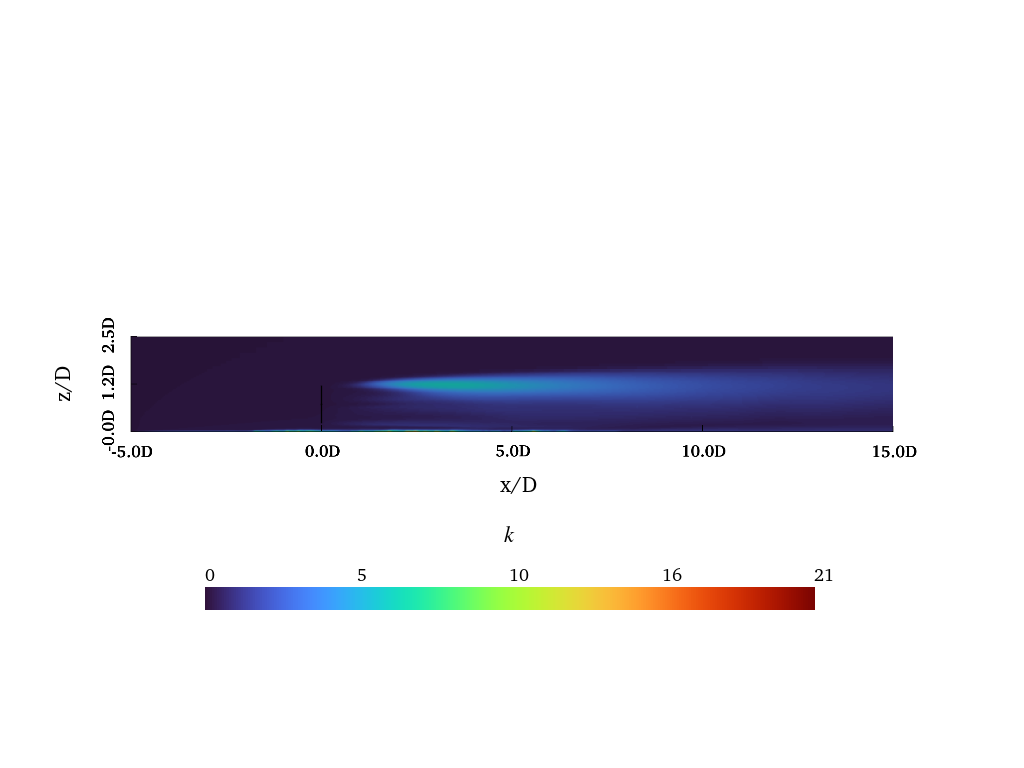
\includegraphics[width=\textwidth, trim=80 120 80 150, clip=true]{results/img/predicted_k_field_xz.png}
        \caption{}
        \label{Fig:k_plot}
    \end{subfigure}
    \begin{subfigure}{0.3\textwidth}
        \centering
        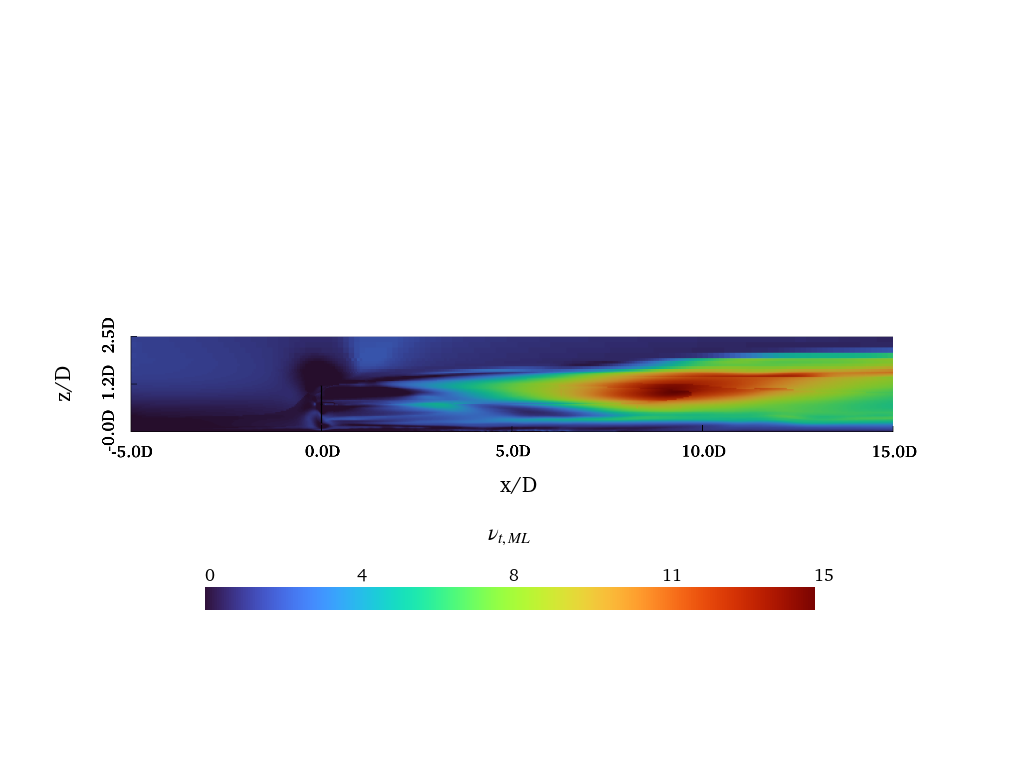
\includegraphics[width=\textwidth, trim=80 120 80 150, clip=true]{results/img/predicted_nut_field_xz.png}
        \caption{}
        \label{Fig:nut_plot}
    \end{subfigure}
    \caption{ML-based RANS model results: (a) velocity deficit along the x-axis at different streamwise distances from the rotor, (b) velocity field, (c) $k$ field, (d) $\nu_{t,ML}$ field.}
    \label{fig:ml_results}
\end{figure}

Velocity deficit along the x-axis at different streamwise distances from the rotor (Fig.~\ref{Fig:velocity_deficit}) is compared, on grids of different resolution, with the standard RANS model and with the LES reference, together with the predicted velocity, turbulent kinetic energy and eddy viscosity fields (Figures \ref{Fig:velocity_plot}-\ref{Fig:nut_plot}).

On the fine grid ($\sim 15.9$ million cells), the ML-based RANS model consistently outperforms the standard RANS model throughout the wake. In the near-wake region the model shows markedly improved agreement with the LES results, especially in the upper region of the wake where the standard RANS model underestimates the velocity deficit. A moderate underestimation of the velocity deficit persists in the lower near-wake region, attributable to a local underestimation of the $\nu_t$. In the far-wake region, after the breakdown of the wake (i.e., from $4D$ in the streamwise direction), the fine-grid model tends to overestimate the velocity deficit with respect to the LES reference, suggesting that at this resolution the $\nu_t$ correction does not fully reproduce the turbulent mixing responsible for wake recovery.

In terms of computational cost, on the $\sim 15.9$ million cells grid the ML-based RANS model is about $2.5$ times more expensive than the reference LES. This figure should not be read as a drawback of the method: the fine grid is not the deployment configuration but the most refined one, retained here only to characterise the accuracy of the closure at high resolution. At this resolution the unsteady time-marching, combined with the per-iteration clustering and network inference, makes the run more expensive than the LES, so the fine-grid comparison is meaningful for accuracy but not for efficiency. The fair efficiency comparison, and the practical advantage of the methodology, emerges on the coarse grids, where LES-quality far-wake accuracy is obtained at a fraction of the LES cost.

The most significant, and practically relevant, result is obtained on the ultra-coarse grids. As shown in Fig.~\ref{Fig:velocity_deficit}, the ML-based RANS model retains its improved near-wake prediction (with lower accuracy with respect to finer grids) while, at the same time, providing a much more accurate description of the far-wake region, including the post-breakdown zone where the fine-grid model overestimates the deficit. This behaviour makes the ultra-coarse configuration the most attractive option for wind farm applications, where an accurate far-wake prediction is critical to estimate the power production of the downstream turbines and to optimise the wind farm layout. The advantage is further reinforced by the reduction in computational cost: on the $\sim 4.2$ million cells grid the ML-based RANS model is about $1.25$ times cheaper than the standard LES, making it a viable tool for large-scale wind farm simulations that require both accuracy and affordability.

Finally, the error in the velocity field is shown in Fig.~\ref{fig:velocity_error_5m} compared to the standard LES model.
\begin{figure}
    \centering
    \begin{subfigure}{0.49\textwidth}
        \centering
        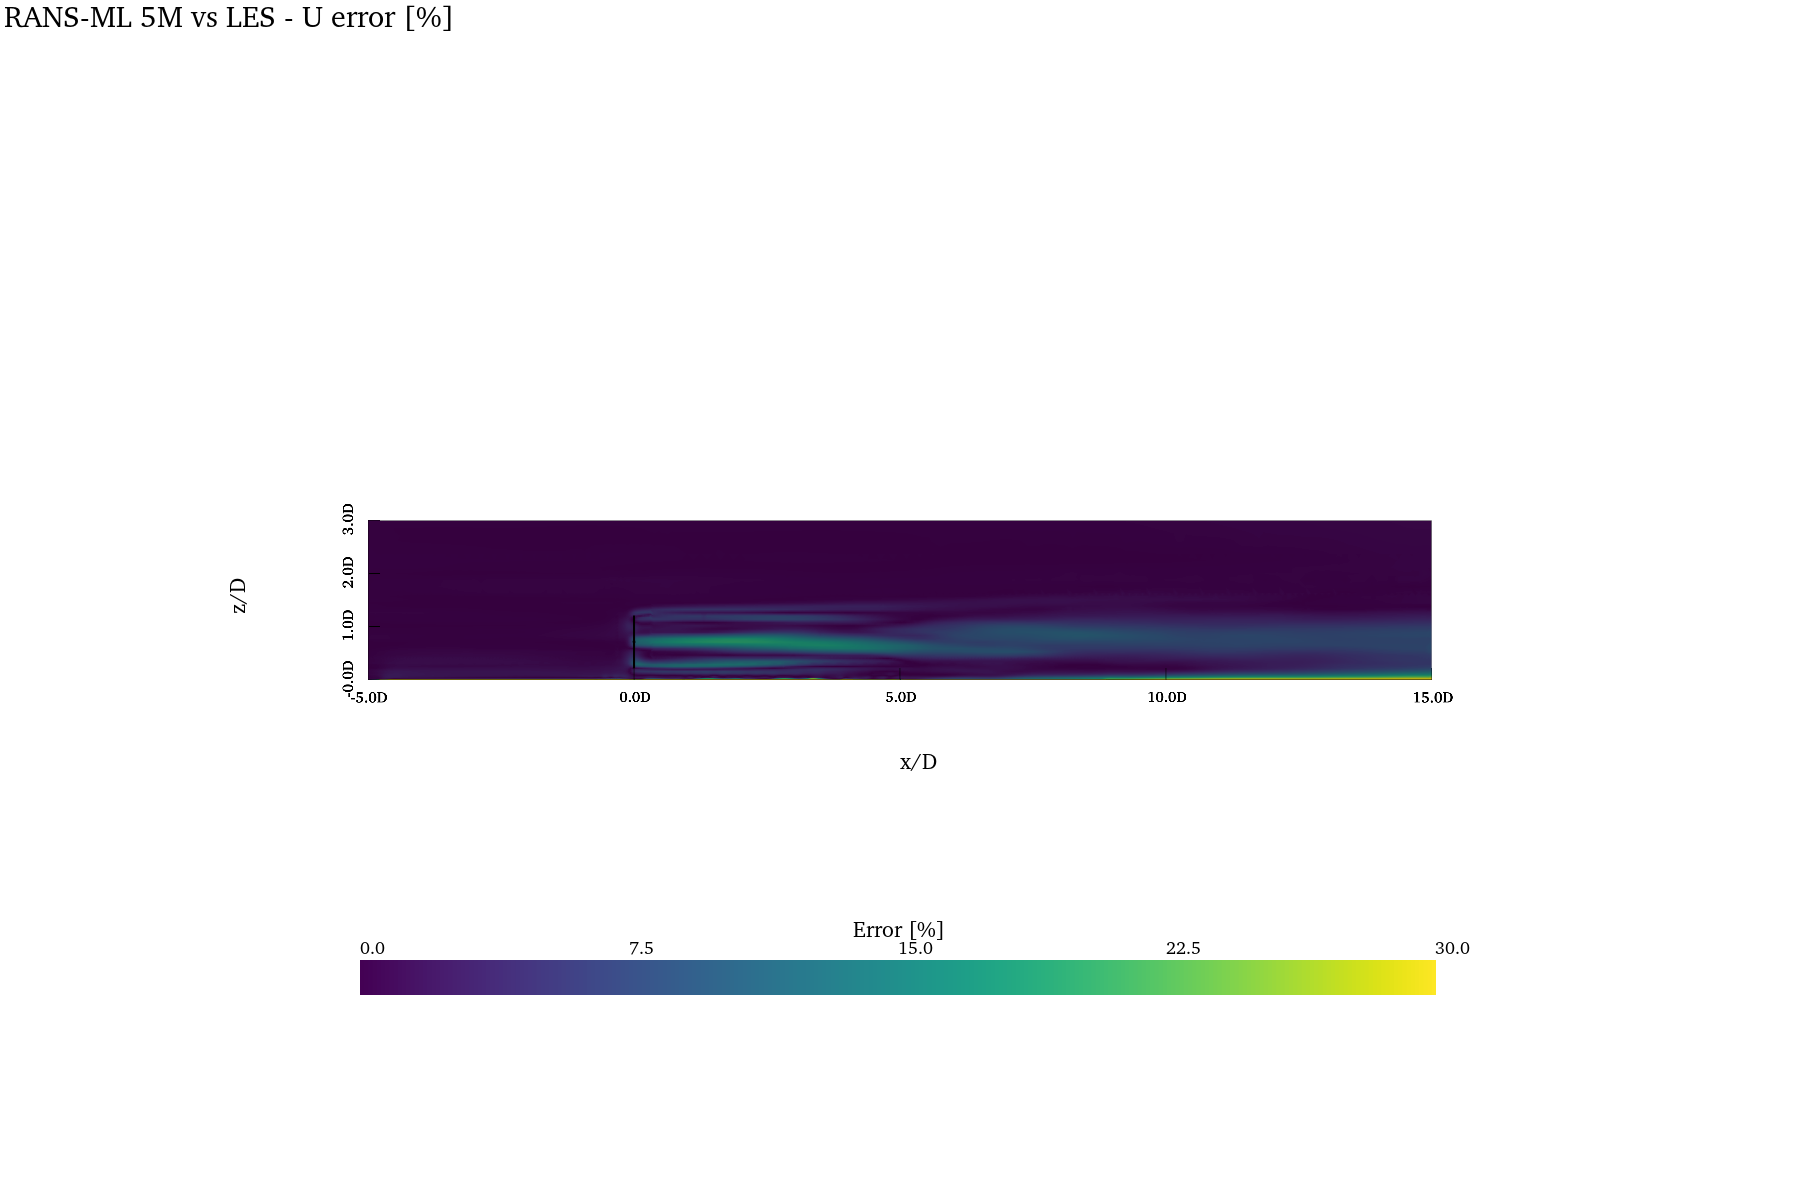
\includegraphics[width=\textwidth, trim=80 120 80 150, clip=true]{results/img/ml_results/11ms/error_fields/rans_ml_5m_vs_les/error_U.png}
        \caption{}
        \label{fig:velocity_error_field_5m}
    \end{subfigure}
    \hfill
    \begin{subfigure}{0.49\textwidth}
        \centering
        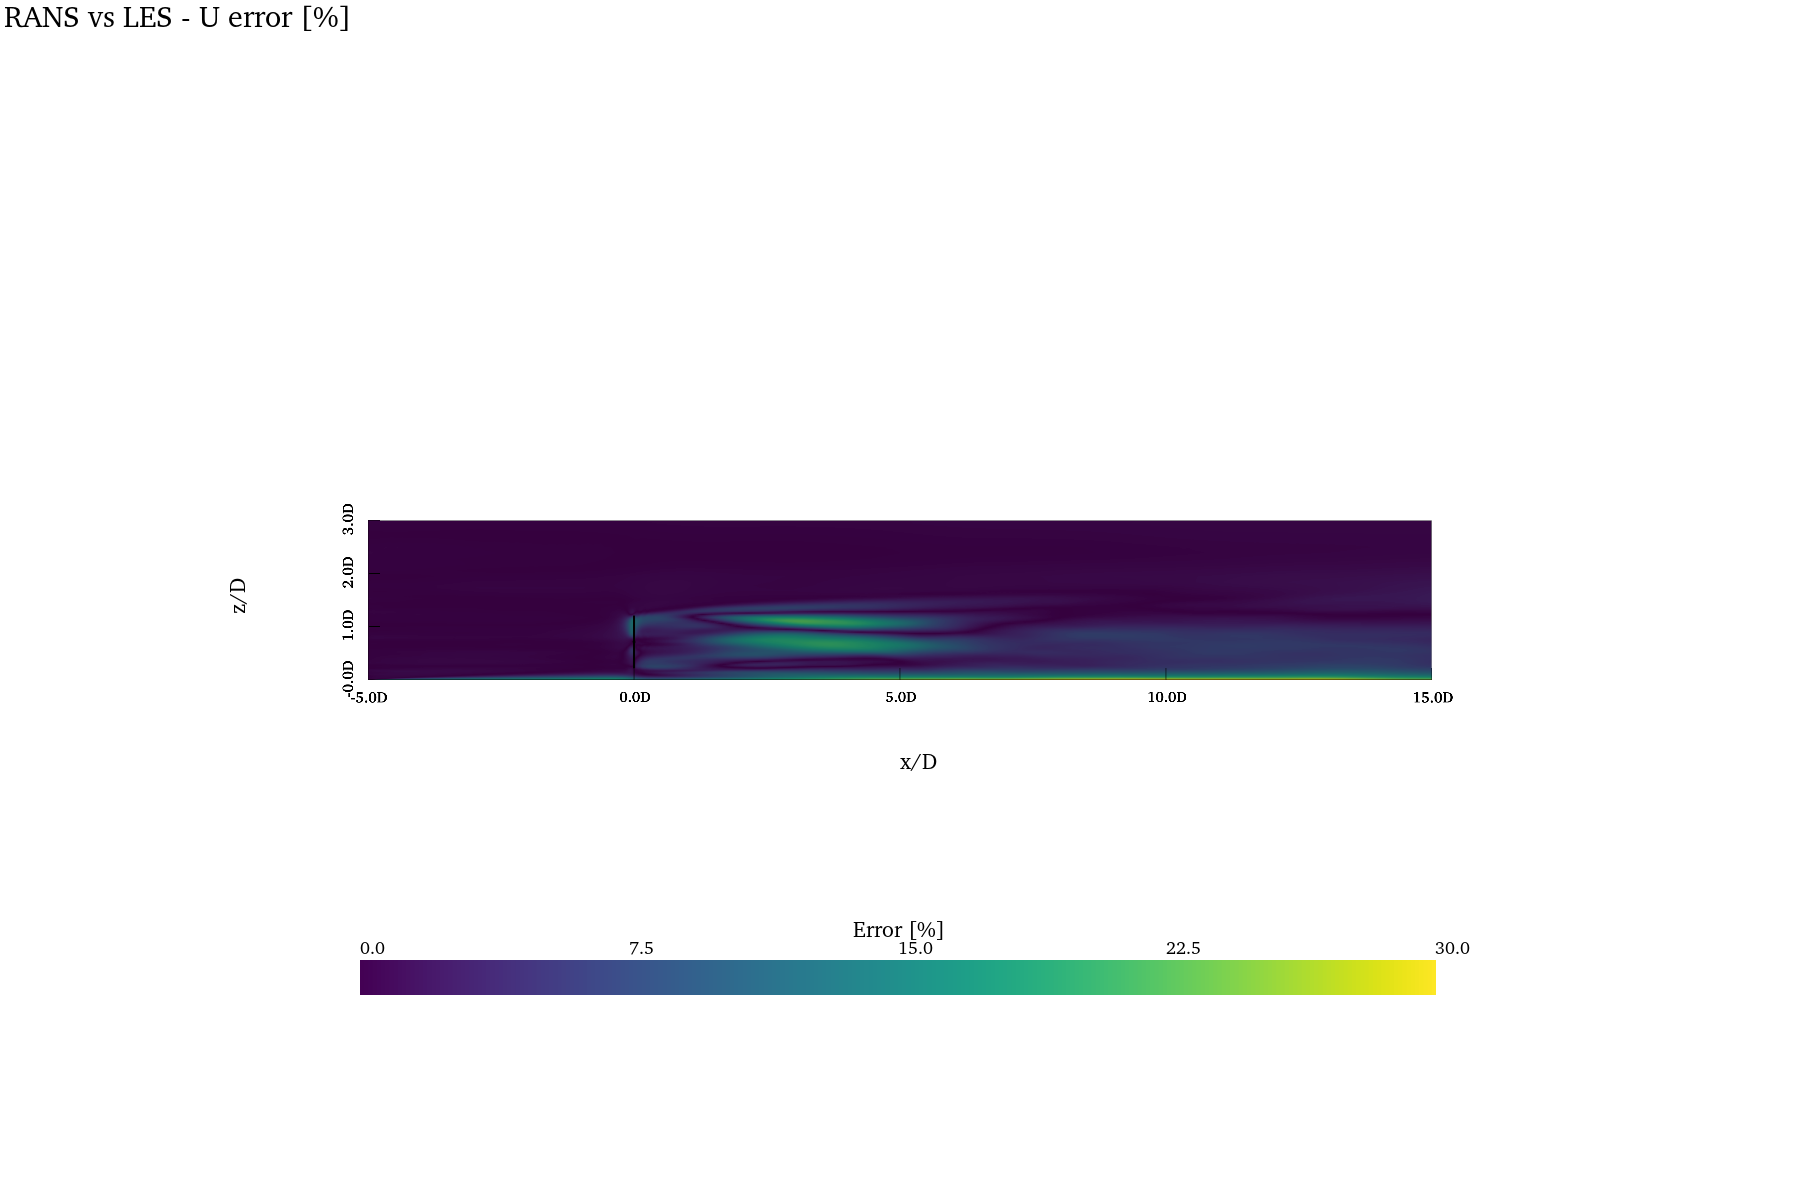
\includegraphics[width=\textwidth, trim=80 120 80 150, clip=true]{results/img/ml_results/11ms/error_fields/rans_vs_les/error_U.png}
        \caption{}
        \label{fig:velocity_error_field_RANS}
    \end{subfigure}
    \caption{Velocity error field of the ML-based RANS model compared to the standard LES model (a) and of RANS one compared to the standard LES model (b).}
    \label{fig:velocity_error_5m}
\end{figure}

The velocity error fields in Fig.~\ref{fig:velocity_error_5m} confirm the trends described above. The ML-based RANS model (Fig.~\ref{fig:velocity_error_field_5m}) achieves a marked reduction of the error in both the near- and far-wake regions with respect to the standard RANS model (Fig.~\ref{fig:velocity_error_field_RANS}), at the cost of a slight increase in the lower part of the near-wake. Importantly, the error in the wake breakdown region is significantly reduced with respect to the standard RANS model, which directly improves the prediction of the wake recovery and is therefore of primary importance for wind farm applications, since wind turbines are usually located in the far-wake region of the upstream machines.

\subsection{Generalization across inflow conditions}
\label{sec:generalization}
Although the network is trained on a single operating condition ($U_\infty=11\,\mathrm{m/s}$), its ability to generalise to unseen inflow velocities is assessed by applying the same closure at $U_\infty=8$ and $15\,\mathrm{m/s}$. To summarise the agreement with the LES reference in a compact way, a scalar metric is defined as the signed integral, across the vertical sampling line, of the difference between the simulated and the LES velocity deficit:
\begin{equation}
    I(x) = \int \left( \frac{\Delta U_{\mathrm{sim}}}{U_\infty} - \frac{\Delta U_{\mathrm{LES}}}{U_\infty} \right) \mathrm{d}\left(\frac{z}{D}\right),
    \label{eq:integral_deficit_difference}
\end{equation}
evaluated at each streamwise station $x/D$, where $\Delta U = U_\infty - |\vec{U}|$ is the velocity deficit. A positive value of $I$ denotes an overall overestimation of the wake deficit (i.e., a slower wake recovery) with respect to the LES, and $I=0$ corresponds to a perfect match of the integrated deficit. Being a signed quantity, $I$ measures the net bias of the wake-deficit prediction at each station: a near-zero $I$ sustained along the whole wake therefore indicates the absence of the systematic over-prediction that affects the standard model, rather than a fortuitous cancellation of local errors, which for the training condition is independently confirmed by the station-by-station profiles of Fig.~\ref{Fig:velocity_deficit}. The resulting trends are reported in Fig.~\ref{fig:integral_deficit_difference} for the three inflow conditions.
\begin{figure}
    \centering
    \begin{subfigure}{0.32\textwidth}
        \centering
        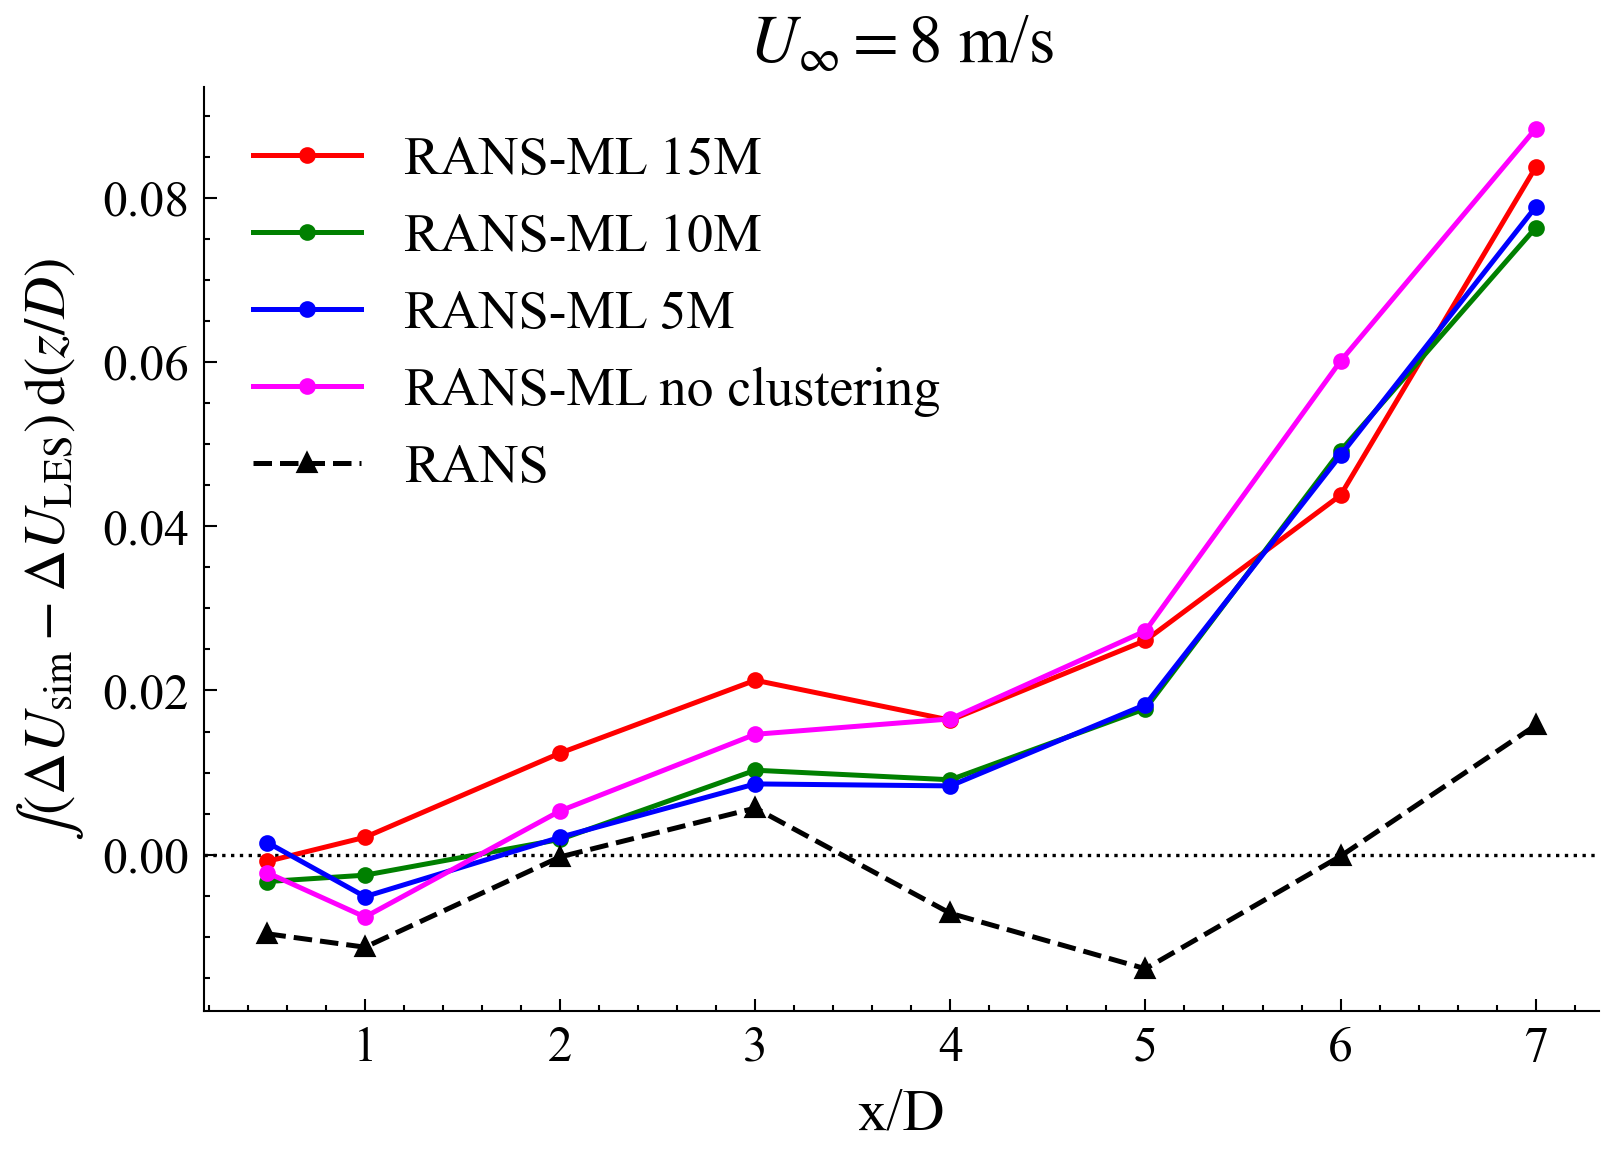
\includegraphics[width=\textwidth]{results/img/ml_results/8ms/integral_deficit_difference.png}
        \caption{}
        \label{fig:integral_8ms}
    \end{subfigure}
    \hfill
    \begin{subfigure}{0.32\textwidth}
        \centering
        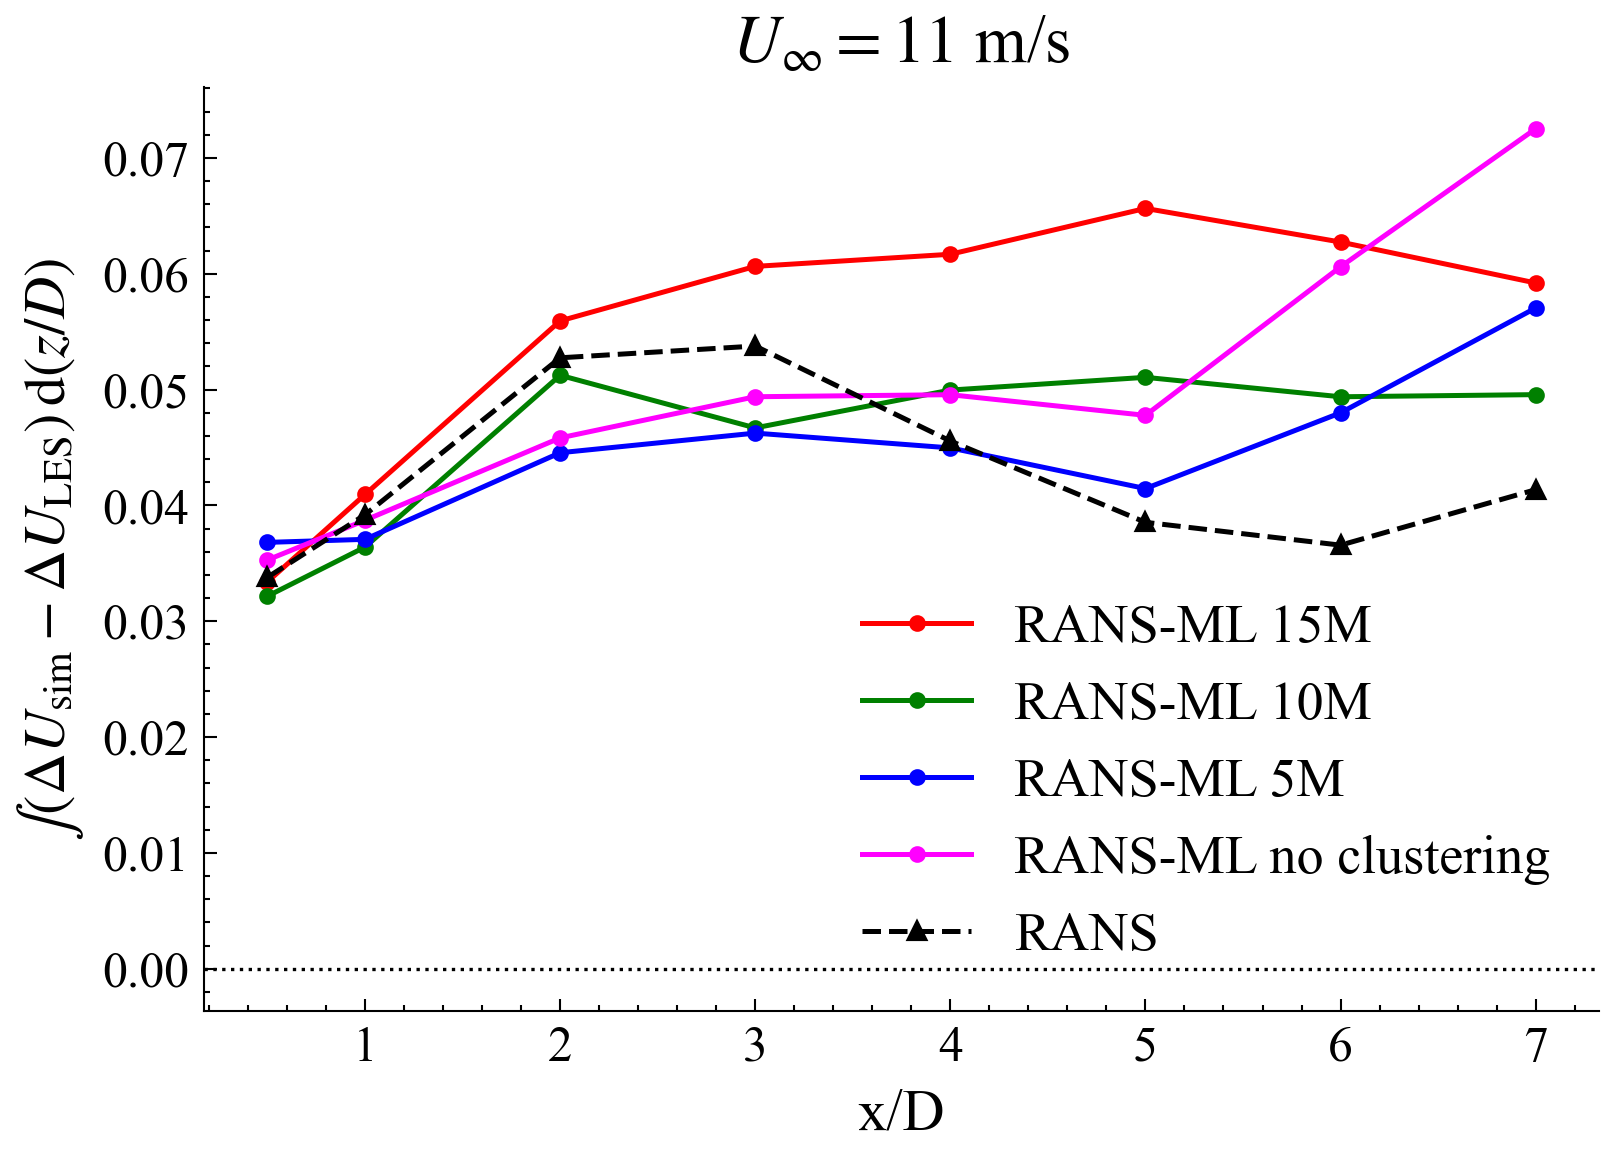
\includegraphics[width=\textwidth]{results/img/ml_results/11ms/integral_deficit_difference.png}
        \caption{}
        \label{fig:integral_11ms}
    \end{subfigure}
    \hfill
    \begin{subfigure}{0.32\textwidth}
        \centering
        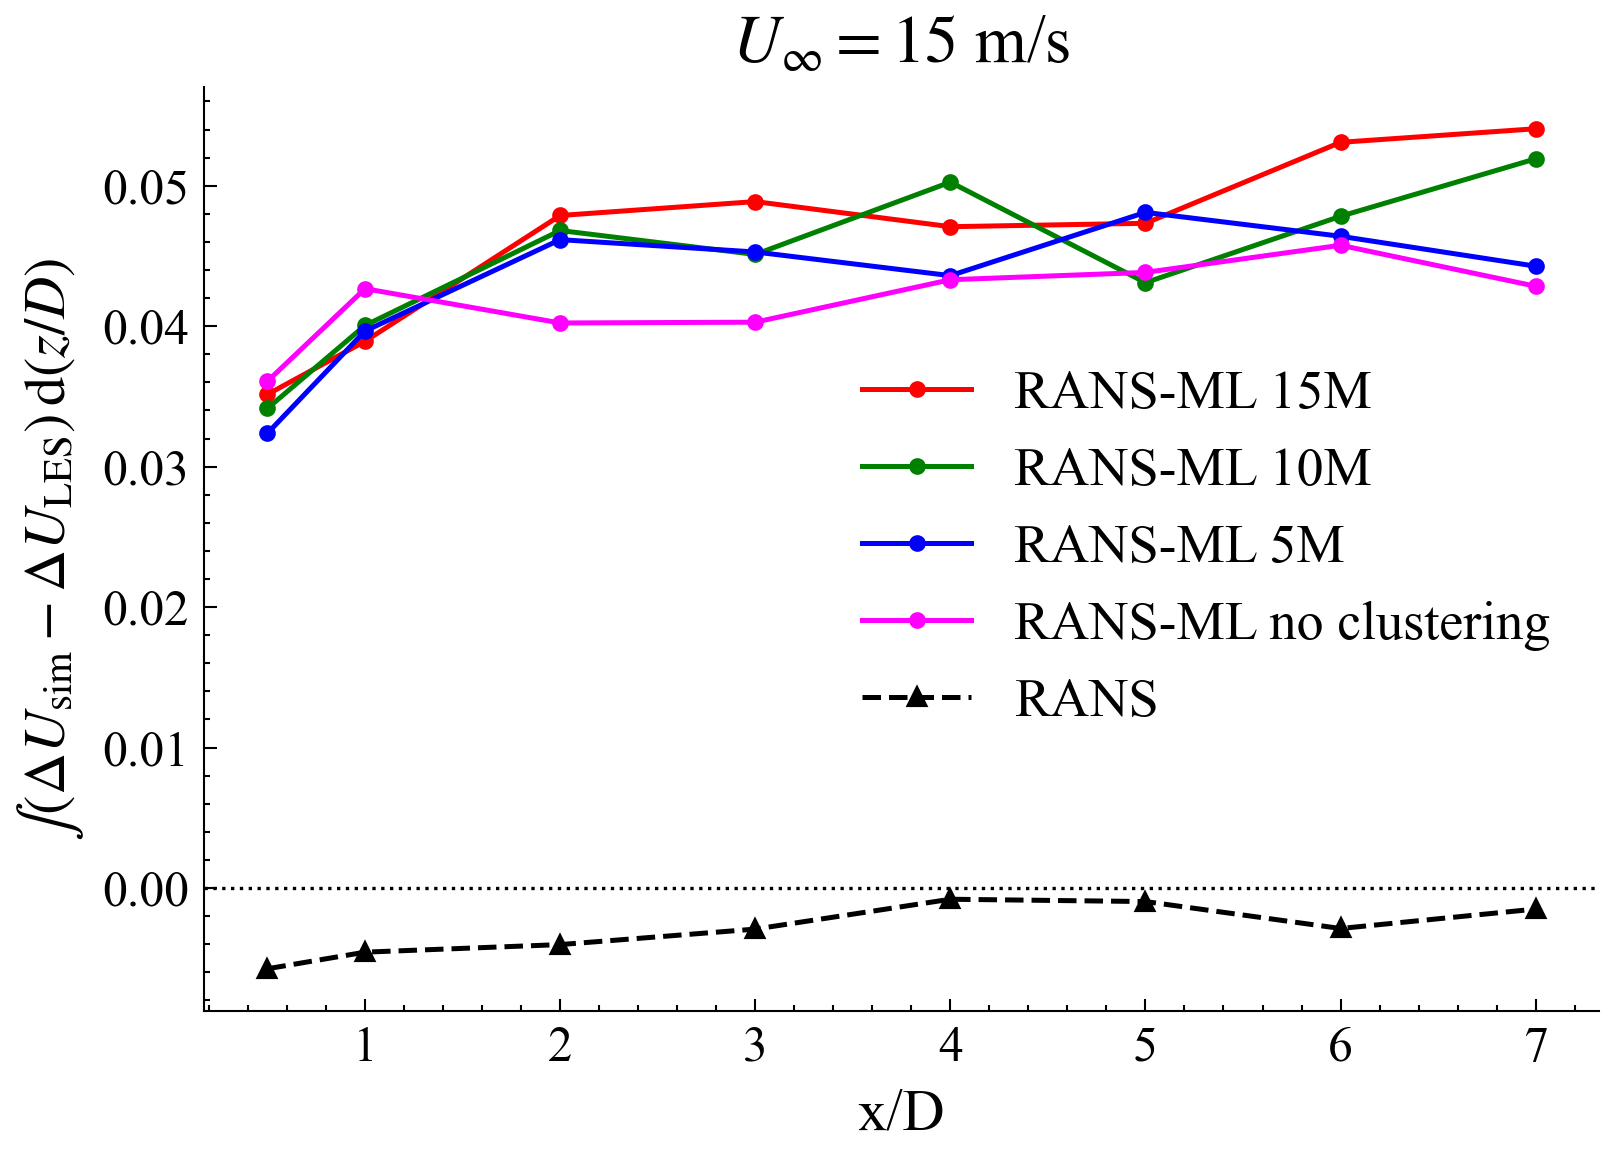
\includegraphics[width=\textwidth]{results/img/ml_results/15ms/integral_deficit_difference.png}
        \caption{}
        \label{fig:integral_15ms}
    \end{subfigure}
    \caption{Signed integral of the velocity-deficit difference with respect to the LES reference, Eq.~\ref{eq:integral_deficit_difference}, as a function of the streamwise distance, for the RANS-ML models on grids of different resolution and for the standard RANS model: (a) $U_\infty=8\,\mathrm{m/s}$, (b) $U_\infty=11\,\mathrm{m/s}$, (c) $U_\infty=15\,\mathrm{m/s}$.}
    \label{fig:integral_deficit_difference}
\end{figure}
For all three inflow velocities the standard RANS model exhibits a large and persistent positive offset throughout the wake, confirming a systematic overestimation of the velocity deficit and an excessively slow wake recovery. In contrast, all the RANS-ML configurations remain close to zero along the whole streamwise extent, even at the inflow conditions ($8$ and $15\,\mathrm{m/s}$) that were not part of the training set. This demonstrates that the learned eddy-viscosity correction is not tied to the specific velocity it was trained on but generalises across different inflow conditions, which is a key requirement for its application to wind farm flows where the operating wind speed varies in time. This is the central evidence supporting the single-case-to-many premise of the methodology: a closure calibrated on one operating point reproduces the LES wake recovery across the inflow envelope, with no retraining and no case-specific tuning.

To assess not only the capability of the model to predict the velocity field but also to investigate its ability to capture the dynamic effects on the wind turbine (and the relative power production), the predicted forces are reported here together with the predicted $C_p$ and $C_t$ values.
\begin{figure}
    \centering
    \begin{subfigure}{0.49\textwidth}
        \centering
        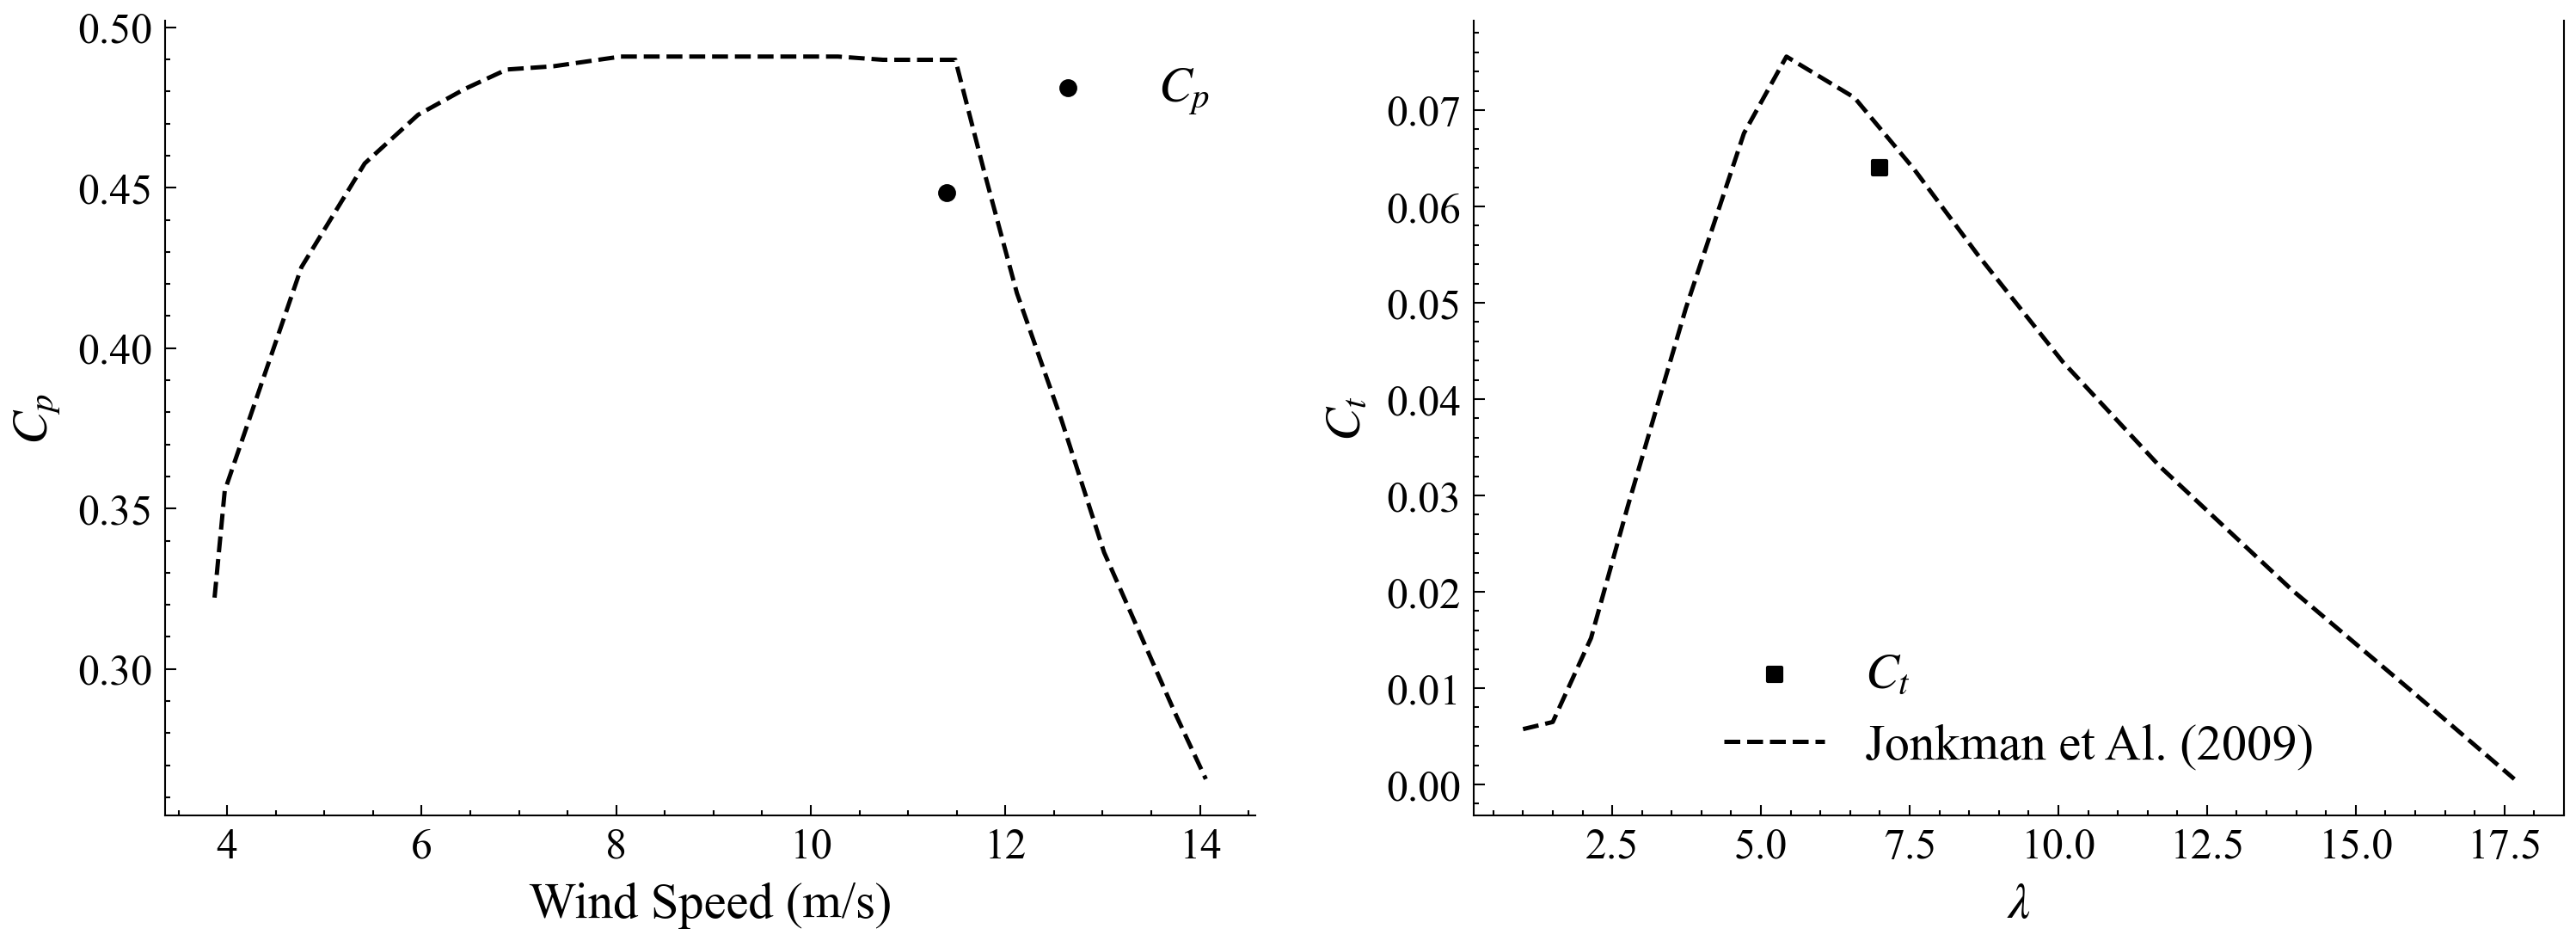
\includegraphics[width=\textwidth]{results/img/forces_cp_ct.png}
        \caption{}
        \label{fig:cp_ct_profile}
    \end{subfigure}
    \hfill
    \begin{subfigure}{0.49\textwidth}
        \centering
        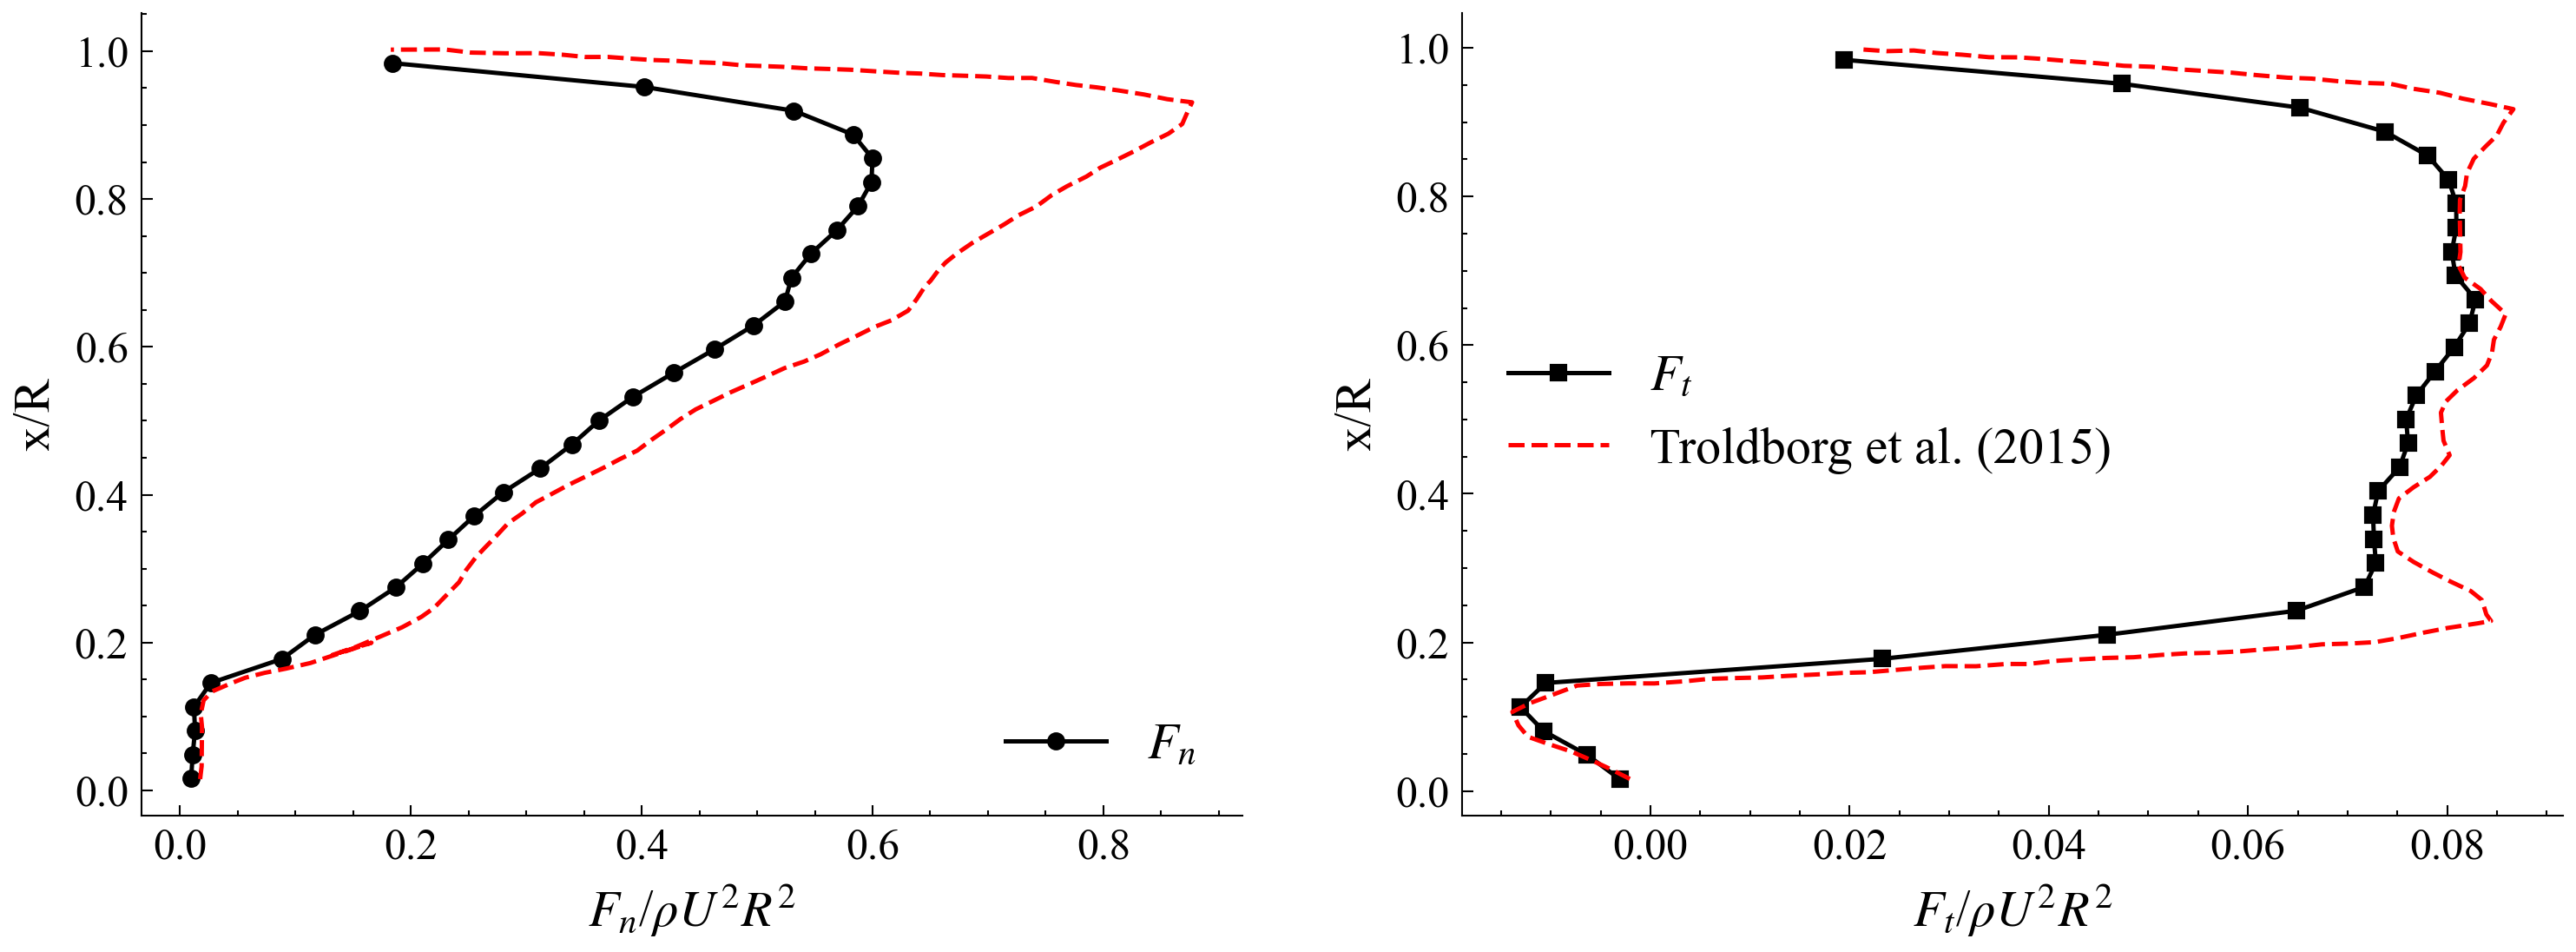
\includegraphics[width=\textwidth]{results/img/forces_profile.png}
        \caption{}
        \label{fig:forces_profile}
    \end{subfigure}
    \caption{ML-based RANS model results on the predicted forces and power coefficients: (a) $C_p$ and $C_t$ profiles, (b) force profiles.}
\end{figure}
The predicted forces show good agreement with the reference curves, with a slight underestimation of the overall forces and coefficients. A small deviation in terms of power production can be noted at the $C_p$ corresponding point; this is partly due to the fact that the reference curves refer to an isolated turbine configuration, whereas the ML-based RANS model is applied to a turbine operating in a turbulent ABL and affected by the presence of the ground. Overall, the predicted forces and power coefficients remain in accordance with the reference curves, demonstrating the capability of the ML-based RANS model to predict not only the velocity wake field but also the dynamic effects on the wind turbine and thus its power production, which is a key aspect for wind farm applications.